% Options for packages loaded elsewhere
\PassOptionsToPackage{unicode}{hyperref}
\PassOptionsToPackage{hyphens}{url}
%
\documentclass[
]{book}
\usepackage{amsmath,amssymb}
\usepackage{iftex}
\ifPDFTeX
  \usepackage[T1]{fontenc}
  \usepackage[utf8]{inputenc}
  \usepackage{textcomp} % provide euro and other symbols
\else % if luatex or xetex
  \usepackage{unicode-math} % this also loads fontspec
  \defaultfontfeatures{Scale=MatchLowercase}
  \defaultfontfeatures[\rmfamily]{Ligatures=TeX,Scale=1}
\fi
\usepackage{lmodern}
\ifPDFTeX\else
  % xetex/luatex font selection
\fi
% Use upquote if available, for straight quotes in verbatim environments
\IfFileExists{upquote.sty}{\usepackage{upquote}}{}
\IfFileExists{microtype.sty}{% use microtype if available
  \usepackage[]{microtype}
  \UseMicrotypeSet[protrusion]{basicmath} % disable protrusion for tt fonts
}{}
\makeatletter
\@ifundefined{KOMAClassName}{% if non-KOMA class
  \IfFileExists{parskip.sty}{%
    \usepackage{parskip}
  }{% else
    \setlength{\parindent}{0pt}
    \setlength{\parskip}{6pt plus 2pt minus 1pt}}
}{% if KOMA class
  \KOMAoptions{parskip=half}}
\makeatother
\usepackage{xcolor}
\usepackage{color}
\usepackage{fancyvrb}
\newcommand{\VerbBar}{|}
\newcommand{\VERB}{\Verb[commandchars=\\\{\}]}
\DefineVerbatimEnvironment{Highlighting}{Verbatim}{commandchars=\\\{\}}
% Add ',fontsize=\small' for more characters per line
\usepackage{framed}
\definecolor{shadecolor}{RGB}{248,248,248}
\newenvironment{Shaded}{\begin{snugshade}}{\end{snugshade}}
\newcommand{\AlertTok}[1]{\textcolor[rgb]{0.94,0.16,0.16}{#1}}
\newcommand{\AnnotationTok}[1]{\textcolor[rgb]{0.56,0.35,0.01}{\textbf{\textit{#1}}}}
\newcommand{\AttributeTok}[1]{\textcolor[rgb]{0.13,0.29,0.53}{#1}}
\newcommand{\BaseNTok}[1]{\textcolor[rgb]{0.00,0.00,0.81}{#1}}
\newcommand{\BuiltInTok}[1]{#1}
\newcommand{\CharTok}[1]{\textcolor[rgb]{0.31,0.60,0.02}{#1}}
\newcommand{\CommentTok}[1]{\textcolor[rgb]{0.56,0.35,0.01}{\textit{#1}}}
\newcommand{\CommentVarTok}[1]{\textcolor[rgb]{0.56,0.35,0.01}{\textbf{\textit{#1}}}}
\newcommand{\ConstantTok}[1]{\textcolor[rgb]{0.56,0.35,0.01}{#1}}
\newcommand{\ControlFlowTok}[1]{\textcolor[rgb]{0.13,0.29,0.53}{\textbf{#1}}}
\newcommand{\DataTypeTok}[1]{\textcolor[rgb]{0.13,0.29,0.53}{#1}}
\newcommand{\DecValTok}[1]{\textcolor[rgb]{0.00,0.00,0.81}{#1}}
\newcommand{\DocumentationTok}[1]{\textcolor[rgb]{0.56,0.35,0.01}{\textbf{\textit{#1}}}}
\newcommand{\ErrorTok}[1]{\textcolor[rgb]{0.64,0.00,0.00}{\textbf{#1}}}
\newcommand{\ExtensionTok}[1]{#1}
\newcommand{\FloatTok}[1]{\textcolor[rgb]{0.00,0.00,0.81}{#1}}
\newcommand{\FunctionTok}[1]{\textcolor[rgb]{0.13,0.29,0.53}{\textbf{#1}}}
\newcommand{\ImportTok}[1]{#1}
\newcommand{\InformationTok}[1]{\textcolor[rgb]{0.56,0.35,0.01}{\textbf{\textit{#1}}}}
\newcommand{\KeywordTok}[1]{\textcolor[rgb]{0.13,0.29,0.53}{\textbf{#1}}}
\newcommand{\NormalTok}[1]{#1}
\newcommand{\OperatorTok}[1]{\textcolor[rgb]{0.81,0.36,0.00}{\textbf{#1}}}
\newcommand{\OtherTok}[1]{\textcolor[rgb]{0.56,0.35,0.01}{#1}}
\newcommand{\PreprocessorTok}[1]{\textcolor[rgb]{0.56,0.35,0.01}{\textit{#1}}}
\newcommand{\RegionMarkerTok}[1]{#1}
\newcommand{\SpecialCharTok}[1]{\textcolor[rgb]{0.81,0.36,0.00}{\textbf{#1}}}
\newcommand{\SpecialStringTok}[1]{\textcolor[rgb]{0.31,0.60,0.02}{#1}}
\newcommand{\StringTok}[1]{\textcolor[rgb]{0.31,0.60,0.02}{#1}}
\newcommand{\VariableTok}[1]{\textcolor[rgb]{0.00,0.00,0.00}{#1}}
\newcommand{\VerbatimStringTok}[1]{\textcolor[rgb]{0.31,0.60,0.02}{#1}}
\newcommand{\WarningTok}[1]{\textcolor[rgb]{0.56,0.35,0.01}{\textbf{\textit{#1}}}}
\usepackage{longtable,booktabs,array}
\usepackage{calc} % for calculating minipage widths
% Correct order of tables after \paragraph or \subparagraph
\usepackage{etoolbox}
\makeatletter
\patchcmd\longtable{\par}{\if@noskipsec\mbox{}\fi\par}{}{}
\makeatother
% Allow footnotes in longtable head/foot
\IfFileExists{footnotehyper.sty}{\usepackage{footnotehyper}}{\usepackage{footnote}}
\makesavenoteenv{longtable}
\usepackage{graphicx}
\makeatletter
\def\maxwidth{\ifdim\Gin@nat@width>\linewidth\linewidth\else\Gin@nat@width\fi}
\def\maxheight{\ifdim\Gin@nat@height>\textheight\textheight\else\Gin@nat@height\fi}
\makeatother
% Scale images if necessary, so that they will not overflow the page
% margins by default, and it is still possible to overwrite the defaults
% using explicit options in \includegraphics[width, height, ...]{}
\setkeys{Gin}{width=\maxwidth,height=\maxheight,keepaspectratio}
% Set default figure placement to htbp
\makeatletter
\def\fps@figure{htbp}
\makeatother
\setlength{\emergencystretch}{3em} % prevent overfull lines
\providecommand{\tightlist}{%
  \setlength{\itemsep}{0pt}\setlength{\parskip}{0pt}}
\setcounter{secnumdepth}{5}
\usepackage{booktabs}
\ifLuaTeX
  \usepackage{selnolig}  % disable illegal ligatures
\fi
\usepackage[]{natbib}
\bibliographystyle{plainnat}
\IfFileExists{bookmark.sty}{\usepackage{bookmark}}{\usepackage{hyperref}}
\IfFileExists{xurl.sty}{\usepackage{xurl}}{} % add URL line breaks if available
\urlstyle{same}
\hypersetup{
  pdftitle={西山ほか(2019)『計量経済学』有斐閣の練習問題解答とRでの再現},
  pdfauthor={石井 俊輔},
  hidelinks,
  pdfcreator={LaTeX via pandoc}}

\title{西山ほか(2019)『計量経済学』有斐閣の練習問題解答とRでの再現}
\author{石井 俊輔}
\date{2024-04-28}

\begin{document}
\maketitle

{
\setcounter{tocdepth}{1}
\tableofcontents
}
\hypertarget{ux306fux3058ux3081ux306b}{%
\chapter*{はじめに}\label{ux306fux3058ux3081ux306b}}
\addcontentsline{toc}{chapter}{はじめに}

西山ほか(2019)『計量経済学』有斐閣 (\href{https://www.yuhikaku.co.jp/books/detail/9784641053854}{出版社リンク}) の練習問題解答とRでの再現です.
必要なRパッケージをインストール:

\begin{Shaded}
\begin{Highlighting}[]
\FunctionTok{install.packages}\NormalTok{(}\StringTok{"tidyverse"}\NormalTok{)}
\FunctionTok{install.packages}\NormalTok{(}\StringTok{"openxlsx"}\NormalTok{)}
\FunctionTok{install.packages}\NormalTok{(}\StringTok{"haven"}\NormalTok{)}
\FunctionTok{install.packages}\NormalTok{(}\StringTok{"wooldridge"}\NormalTok{)}
\FunctionTok{install.packages}\NormalTok{(}\StringTok{"fixest"}\NormalTok{)}
\end{Highlighting}
\end{Shaded}

\hypertarget{usage}{%
\section{Usage}\label{usage}}

Each \textbf{bookdown} chapter is an .Rmd file, and each .Rmd file can contain one (and only one) chapter. A chapter \emph{must} start with a first-level heading: \texttt{\#\ A\ good\ chapter}, and can contain one (and only one) first-level heading.

Use second-level and higher headings within chapters like: \texttt{\#\#\ A\ short\ section} or \texttt{\#\#\#\ An\ even\ shorter\ section}.

The \texttt{index.Rmd} file is required, and is also your first book chapter. It will be the homepage when you render the book.

\hypertarget{render-book}{%
\section{Render book}\label{render-book}}

You can render the HTML version of this example book without changing anything:

\begin{enumerate}
\def\labelenumi{\arabic{enumi}.}
\item
  Find the \textbf{Build} pane in the RStudio IDE, and
\item
  Click on \textbf{Build Book}, then select your output format, or select ``All formats'' if you'd like to use multiple formats from the same book source files.
\end{enumerate}

Or build the book from the R console:

\begin{Shaded}
\begin{Highlighting}[]
\NormalTok{bookdown}\SpecialCharTok{::}\FunctionTok{render\_book}\NormalTok{()}
\end{Highlighting}
\end{Shaded}

To render this example to PDF as a \texttt{bookdown::pdf\_book}, you'll need to install XeLaTeX. You are recommended to install TinyTeX (which includes XeLaTeX): \url{https://yihui.org/tinytex/}.

\hypertarget{preview-book}{%
\section{Preview book}\label{preview-book}}

As you work, you may start a local server to live preview this HTML book. This preview will update as you edit the book when you save individual .Rmd files. You can start the server in a work session by using the RStudio add-in ``Preview book'', or from the R console:

\begin{Shaded}
\begin{Highlighting}[]
\NormalTok{bookdown}\SpecialCharTok{::}\FunctionTok{serve\_book}\NormalTok{()}
\end{Highlighting}
\end{Shaded}

\hypertarget{ch2}{%
\chapter*{第2章 データの整理と確率変数の基礎}\label{ch2}}
\addcontentsline{toc}{chapter}{第2章 データの整理と確率変数の基礎}

先に\href{https://www.yuhikaku.co.jp/books/detail/9784641053854}{出版社サイト}よりデータをダウンロードする.

\begin{Shaded}
\begin{Highlighting}[]
\CommentTok{\# サポートファイルへのリンク}
\NormalTok{curl }\OtherTok{\textless{}{-}} \StringTok{"https://www.yuhikaku.co.jp/static\_files/05385\_support02.zip"}
\CommentTok{\# ダウンロード保存用フォルダが存在しない場合, 作成}
\ControlFlowTok{if}\NormalTok{(}\SpecialCharTok{!}\FunctionTok{dir.exists}\NormalTok{(}\StringTok{"downloads"}\NormalTok{))\{}
    \FunctionTok{dir.create}\NormalTok{(}\StringTok{"downloads"}\NormalTok{)}
\NormalTok{\}}
\NormalTok{cdestfile }\OtherTok{\textless{}{-}} \StringTok{"downloads/support02.zip"}
\FunctionTok{download.file}\NormalTok{(curl, cdestfile)}
\CommentTok{\# データ保存用フォルダが存在しない場合, 作成}
\ControlFlowTok{if}\NormalTok{(}\SpecialCharTok{!}\FunctionTok{dir.exists}\NormalTok{(}\StringTok{"data"}\NormalTok{))\{}
    \FunctionTok{dir.create}\NormalTok{(}\StringTok{"data"}\NormalTok{)}
\NormalTok{\}}
\CommentTok{\# WSL上のRで解凍すると文字化けするので、Linuxのコマンドを外部呼び出し}
\CommentTok{\# Windowsの場合は別途コマンドを用いる.}
\ControlFlowTok{if}\NormalTok{(.Platform}\SpecialCharTok{$}\NormalTok{OS.type }\SpecialCharTok{==} \StringTok{"unix"}\NormalTok{) \{}
    \FunctionTok{system}\NormalTok{(}\FunctionTok{sprintf}\NormalTok{(}\StringTok{\textquotesingle{}unzip {-}n {-}Ocp932 \%s {-}d \%s\textquotesingle{}}\NormalTok{, }\StringTok{"downloads/support02.zip"}\NormalTok{, }\StringTok{"./data"}\NormalTok{))}
\NormalTok{\} }\ControlFlowTok{else}\NormalTok{ \{}
    \FunctionTok{print}\NormalTok{(}\StringTok{"Windowsで解凍するコマンドを別途追加せよ."}\NormalTok{)}
\NormalTok{\}}
\end{Highlighting}
\end{Shaded}

必要なライブラリを読み込む.

\begin{Shaded}
\begin{Highlighting}[]
\FunctionTok{library}\NormalTok{(tidyverse)}
\DocumentationTok{\#\# {-}{-} Attaching core tidyverse packages {-}{-}{-}{-}{-}{-}{-}{-}{-}{-}{-}{-}{-}{-}{-}{-}{-}{-}{-}{-}{-}{-}{-}{-} tidyverse 2.0.0 {-}{-}}
\DocumentationTok{\#\# v dplyr     1.1.4     v readr     2.1.5}
\DocumentationTok{\#\# v forcats   1.0.0     v stringr   1.5.1}
\DocumentationTok{\#\# v ggplot2   3.5.0     v tibble    3.2.1}
\DocumentationTok{\#\# v lubridate 1.9.3     v tidyr     1.3.1}
\DocumentationTok{\#\# v purrr     1.0.2     }
\DocumentationTok{\#\# {-}{-} Conflicts {-}{-}{-}{-}{-}{-}{-}{-}{-}{-}{-}{-}{-}{-}{-}{-}{-}{-}{-}{-}{-}{-}{-}{-}{-}{-}{-}{-}{-}{-}{-}{-}{-}{-}{-}{-}{-}{-}{-}{-}{-}{-} tidyverse\_conflicts() {-}{-}}
\DocumentationTok{\#\# x dplyr::filter() masks stats::filter()}
\DocumentationTok{\#\# x dplyr::lag()    masks stats::lag()}
\DocumentationTok{\#\# i Use the conflicted package (\textless{}http://conflicted.r{-}lib.org/\textgreater{}) to force all conflicts to become errors}
\end{Highlighting}
\end{Shaded}

\hypertarget{ux7df4ux7fd2ux554fux984c-2-1-ux78baux8a8d}{%
\section*{練習問題 2-1 {[}確認{]}}\label{ux7df4ux7fd2ux554fux984c-2-1-ux78baux8a8d}}
\addcontentsline{toc}{section}{練習問題 2-1 {[}確認{]}}

R には最頻値を求める関数がないようなので, 別途関数\texttt{Mode()}を定義する.

\begin{Shaded}
\begin{Highlighting}[]
\NormalTok{data21 }\OtherTok{\textless{}{-}} \FunctionTok{read.table}\NormalTok{(}\StringTok{"data/02\_第2章/02\_practice\_01.csv"}\NormalTok{)}

\FunctionTok{mean}\NormalTok{(data21}\SpecialCharTok{$}\NormalTok{V1)}
\DocumentationTok{\#\# [1] 10}
\FunctionTok{var}\NormalTok{(data21}\SpecialCharTok{$}\NormalTok{V1)}
\DocumentationTok{\#\# [1] 18.10526}
\FunctionTok{median}\NormalTok{(data21}\SpecialCharTok{$}\NormalTok{V1)}
\DocumentationTok{\#\# [1] 10}

\NormalTok{Mode }\OtherTok{\textless{}{-}} \ControlFlowTok{function}\NormalTok{(x) \{}
\NormalTok{    ux }\OtherTok{\textless{}{-}} \FunctionTok{unique}\NormalTok{(x)}
\NormalTok{    tab }\OtherTok{\textless{}{-}} \FunctionTok{tabulate}\NormalTok{(}\FunctionTok{match}\NormalTok{(x, ux))}
\NormalTok{    ux[tab }\SpecialCharTok{==} \FunctionTok{max}\NormalTok{(tab)]}
\NormalTok{\}}

\FunctionTok{Mode}\NormalTok{(data21}\SpecialCharTok{$}\NormalTok{V1)}
\DocumentationTok{\#\# [1] 10}
\end{Highlighting}
\end{Shaded}

\hypertarget{ux7df4ux7fd2ux554fux984c-2-2-ux78baux8a8d}{%
\section*{練習問題 2-2 {[}確認{]}}\label{ux7df4ux7fd2ux554fux984c-2-2-ux78baux8a8d}}
\addcontentsline{toc}{section}{練習問題 2-2 {[}確認{]}}

\hypertarget{ux7df4ux7fd2ux554fux984c-2-3-ux78baux8a8d}{%
\section*{練習問題 2-3 {[}確認{]}}\label{ux7df4ux7fd2ux554fux984c-2-3-ux78baux8a8d}}
\addcontentsline{toc}{section}{練習問題 2-3 {[}確認{]}}

\begin{Shaded}
\begin{Highlighting}[]
\NormalTok{data23 }\OtherTok{\textless{}{-}} \FunctionTok{read.table}\NormalTok{(}\StringTok{"data/02\_第2章/02\_practice\_03.csv"}\NormalTok{, }\AttributeTok{sep=}\StringTok{","}\NormalTok{)}

\NormalTok{x }\OtherTok{\textless{}{-}}\NormalTok{ data23}\SpecialCharTok{$}\NormalTok{V1}
\NormalTok{y }\OtherTok{\textless{}{-}}\NormalTok{ data23}\SpecialCharTok{$}\NormalTok{V2}

\NormalTok{data23 }\SpecialCharTok{\%\textgreater{}\%}
    \FunctionTok{ggplot}\NormalTok{(}\FunctionTok{aes}\NormalTok{(}\AttributeTok{x =}\NormalTok{ x, }\AttributeTok{y =}\NormalTok{ y)) }\SpecialCharTok{+}
    \FunctionTok{geom\_point}\NormalTok{()}
\end{Highlighting}
\end{Shaded}

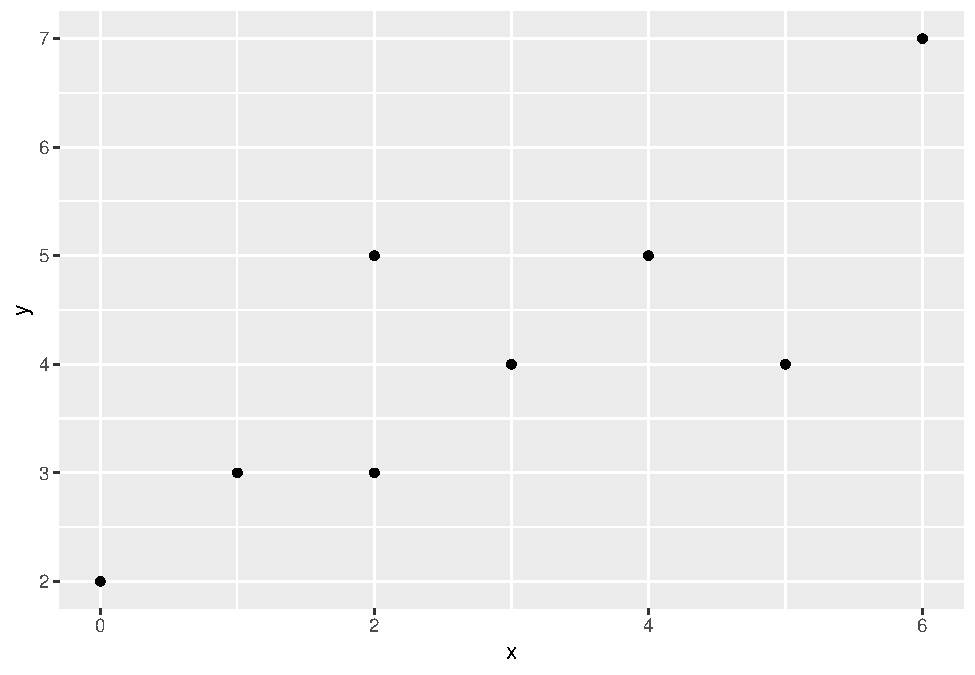
\includegraphics{_main_files/figure-latex/unnamed-chunk-8-1.pdf}

\begin{Shaded}
\begin{Highlighting}[]

\FunctionTok{cov}\NormalTok{(x, y)}
\DocumentationTok{\#\# [1] 2.111111}
\FunctionTok{cor}\NormalTok{(x, y)}
\DocumentationTok{\#\# [1] 0.7680295}
\end{Highlighting}
\end{Shaded}

\hypertarget{ux7df4ux7fd2ux554fux984c-2-4-ux78baux8a8d}{%
\section*{練習問題 2-4 {[}確認{]}}\label{ux7df4ux7fd2ux554fux984c-2-4-ux78baux8a8d}}
\addcontentsline{toc}{section}{練習問題 2-4 {[}確認{]}}

\hypertarget{ux7df4ux7fd2ux554fux984c-2-5-ux78baux8a8d}{%
\section*{練習問題 2-5 {[}確認{]}}\label{ux7df4ux7fd2ux554fux984c-2-5-ux78baux8a8d}}
\addcontentsline{toc}{section}{練習問題 2-5 {[}確認{]}}

\hypertarget{ux7df4ux7fd2ux554fux984c-2-6-ux78baux8a8d}{%
\section*{練習問題 2-6 {[}確認{]}}\label{ux7df4ux7fd2ux554fux984c-2-6-ux78baux8a8d}}
\addcontentsline{toc}{section}{練習問題 2-6 {[}確認{]}}

\hypertarget{ux7df4ux7fd2ux554fux984c-2-7-ux767aux5c55}{%
\section*{練習問題 2-7 {[}発展{]}}\label{ux7df4ux7fd2ux554fux984c-2-7-ux767aux5c55}}
\addcontentsline{toc}{section}{練習問題 2-7 {[}発展{]}}

\hypertarget{ux7df4ux7fd2ux554fux984c-2-8-ux767aux5c55}{%
\section*{練習問題 2-8 {[}発展{]}}\label{ux7df4ux7fd2ux554fux984c-2-8-ux767aux5c55}}
\addcontentsline{toc}{section}{練習問題 2-8 {[}発展{]}}

\hypertarget{ux7df4ux7fd2ux554fux984c-2-9-ux767aux5c55}{%
\section*{練習問題 2-9 {[}発展{]}}\label{ux7df4ux7fd2ux554fux984c-2-9-ux767aux5c55}}
\addcontentsline{toc}{section}{練習問題 2-9 {[}発展{]}}

\hypertarget{ux7df4ux7fd2ux554fux984c-2-10-ux767aux5c55}{%
\section*{練習問題 2-10 {[}発展{]}}\label{ux7df4ux7fd2ux554fux984c-2-10-ux767aux5c55}}
\addcontentsline{toc}{section}{練習問題 2-10 {[}発展{]}}

\hypertarget{ux7df4ux7fd2ux554fux984c-2-11-ux78baux8a8d}{%
\section*{練習問題 2-11 {[}確認{]}}\label{ux7df4ux7fd2ux554fux984c-2-11-ux78baux8a8d}}
\addcontentsline{toc}{section}{練習問題 2-11 {[}確認{]}}

\hypertarget{ux7df4ux7fd2ux554fux984c-2-12-ux767aux5c55}{%
\section*{練習問題 2-12 {[}発展{]}}\label{ux7df4ux7fd2ux554fux984c-2-12-ux767aux5c55}}
\addcontentsline{toc}{section}{練習問題 2-12 {[}発展{]}}

\hypertarget{ux7df4ux7fd2ux554fux984c-2-13-ux78baux8a8d}{%
\section*{練習問題 2-13 {[}確認{]}}\label{ux7df4ux7fd2ux554fux984c-2-13-ux78baux8a8d}}
\addcontentsline{toc}{section}{練習問題 2-13 {[}確認{]}}

\hypertarget{ux7df4ux7fd2ux554fux984c-2-14-ux78baux8a8d}{%
\section*{練習問題 2-14 {[}確認{]}}\label{ux7df4ux7fd2ux554fux984c-2-14-ux78baux8a8d}}
\addcontentsline{toc}{section}{練習問題 2-14 {[}確認{]}}

\hypertarget{ch3}{%
\chapter*{第3章 統計理論の基礎}\label{ch3}}
\addcontentsline{toc}{chapter}{第3章 統計理論の基礎}

第3章では第2章と同じデータを使うため、新たなダウンロードは不要.
なお\href{https://www.yuhikaku.co.jp/books/detail/9784641053854}{出版社サイト}にある第3章のファイルは, 練習問題2-1のデータを用いるところが, 誤って練習問題2-3と同じデータが格納されている.

必要なライブラリを読み込む.

\begin{Shaded}
\begin{Highlighting}[]
\FunctionTok{library}\NormalTok{(tidyverse)}
\end{Highlighting}
\end{Shaded}

\hypertarget{ux7df4ux7fd2ux554fux984c-3-1-ux78baux8a8d}{%
\section*{練習問題 3-1 {[}確認{]}}\label{ux7df4ux7fd2ux554fux984c-3-1-ux78baux8a8d}}
\addcontentsline{toc}{section}{練習問題 3-1 {[}確認{]}}

\hypertarget{ux7df4ux7fd2ux554fux984c-3-2-ux78baux8a8d}{%
\section*{練習問題 3-2 {[}確認{]}}\label{ux7df4ux7fd2ux554fux984c-3-2-ux78baux8a8d}}
\addcontentsline{toc}{section}{練習問題 3-2 {[}確認{]}}

第2章練習問題2-1で用いたデータを読み込み、両側t検定を実行する.
\(\alpha=0.10\)の場合90\%信頼区間は\([8.354811, 11.645189]\)となり, これは8を含まないことから帰無仮説は棄却できる.
一方で\(\alpha=0.01\)のとき、99\%信頼区間は\([7.277955, 12.722045]\)となり8を含むことから, 帰無仮説は棄却されない.

\begin{Shaded}
\begin{Highlighting}[]
\NormalTok{data32 }\OtherTok{\textless{}{-}} \FunctionTok{read.table}\NormalTok{(}\StringTok{"data/02\_第2章/02\_practice\_01.csv"}\NormalTok{)}
\NormalTok{x }\OtherTok{\textless{}{-}}\NormalTok{ data32}\SpecialCharTok{$}\NormalTok{V1}

\FunctionTok{t.test}\NormalTok{(x, }\AttributeTok{alternative =} \StringTok{"two.sided"}\NormalTok{, }\AttributeTok{mu =} \DecValTok{8}\NormalTok{, }\AttributeTok{conf.level =} \FloatTok{0.90}\NormalTok{)}
\DocumentationTok{\#\# }
\DocumentationTok{\#\#  One Sample t{-}test}
\DocumentationTok{\#\# }
\DocumentationTok{\#\# data:  x}
\DocumentationTok{\#\# t = 2.102, df = 19, p{-}value = 0.04911}
\DocumentationTok{\#\# alternative hypothesis: true mean is not equal to 8}
\DocumentationTok{\#\# 90 percent confidence interval:}
\DocumentationTok{\#\#   8.354811 11.645189}
\DocumentationTok{\#\# sample estimates:}
\DocumentationTok{\#\# mean of x }
\DocumentationTok{\#\#        10}

\FunctionTok{t.test}\NormalTok{(x, }\AttributeTok{alternative =} \StringTok{"two.sided"}\NormalTok{, }\AttributeTok{mu =} \DecValTok{8}\NormalTok{, }\AttributeTok{conf.level =} \FloatTok{0.99}\NormalTok{)}
\DocumentationTok{\#\# }
\DocumentationTok{\#\#  One Sample t{-}test}
\DocumentationTok{\#\# }
\DocumentationTok{\#\# data:  x}
\DocumentationTok{\#\# t = 2.102, df = 19, p{-}value = 0.04911}
\DocumentationTok{\#\# alternative hypothesis: true mean is not equal to 8}
\DocumentationTok{\#\# 99 percent confidence interval:}
\DocumentationTok{\#\#   7.277955 12.722045}
\DocumentationTok{\#\# sample estimates:}
\DocumentationTok{\#\# mean of x }
\DocumentationTok{\#\#        10}
\end{Highlighting}
\end{Shaded}

\hypertarget{ux7df4ux7fd2ux554fux984c-3-3-ux78baux8a8d}{%
\section*{練習問題 3-3 {[}確認{]}}\label{ux7df4ux7fd2ux554fux984c-3-3-ux78baux8a8d}}
\addcontentsline{toc}{section}{練習問題 3-3 {[}確認{]}}

\hypertarget{ux7df4ux7fd2ux554fux984c-3-4-ux767aux5c55}{%
\section*{練習問題 3-4 {[}発展{]}}\label{ux7df4ux7fd2ux554fux984c-3-4-ux767aux5c55}}
\addcontentsline{toc}{section}{練習問題 3-4 {[}発展{]}}

\hypertarget{ch4}{%
\chapter*{第4章 線形単回帰モデルの推定と検定}\label{ch4}}
\addcontentsline{toc}{chapter}{第4章 線形単回帰モデルの推定と検定}

先に\href{https://www.yuhikaku.co.jp/books/detail/9784641053854}{出版社サイト}よりデータをダウンロードする.

\begin{Shaded}
\begin{Highlighting}[]
\CommentTok{\# サポートファイルへのリンク}
\NormalTok{curl }\OtherTok{\textless{}{-}} \StringTok{"https://www.yuhikaku.co.jp/static\_files/05385\_support04.zip"}
\CommentTok{\# ダウンロード保存用フォルダが存在しない場合, 作成}
\ControlFlowTok{if}\NormalTok{(}\SpecialCharTok{!}\FunctionTok{dir.exists}\NormalTok{(}\StringTok{"downloads"}\NormalTok{))\{}
    \FunctionTok{dir.create}\NormalTok{(}\StringTok{"downloads"}\NormalTok{)}
\NormalTok{\}}
\NormalTok{cdestfile }\OtherTok{\textless{}{-}} \StringTok{"downloads/support04.zip"}
\FunctionTok{download.file}\NormalTok{(curl, cdestfile)}
\CommentTok{\# データ保存用フォルダが存在しない場合, 作成}
\ControlFlowTok{if}\NormalTok{(}\SpecialCharTok{!}\FunctionTok{dir.exists}\NormalTok{(}\StringTok{"data"}\NormalTok{))\{}
    \FunctionTok{dir.create}\NormalTok{(}\StringTok{"data"}\NormalTok{)}
\NormalTok{\}}
\CommentTok{\# WSL上のRで解凍すると文字化けするので、Linuxのコマンドを外部呼び出し}
\CommentTok{\# Windowsの場合は別途コマンドを用いる.}
\ControlFlowTok{if}\NormalTok{(.Platform}\SpecialCharTok{$}\NormalTok{OS.type }\SpecialCharTok{==} \StringTok{"unix"}\NormalTok{) \{}
    \FunctionTok{system}\NormalTok{(}\FunctionTok{sprintf}\NormalTok{(}\StringTok{\textquotesingle{}unzip {-}n {-}Ocp932 \%s {-}d \%s\textquotesingle{}}\NormalTok{, }\StringTok{"downloads/support04.zip"}\NormalTok{, }\StringTok{"./data"}\NormalTok{))}
\NormalTok{\} }\ControlFlowTok{else}\NormalTok{ \{}
    \FunctionTok{print}\NormalTok{(}\StringTok{"Windowsで解凍するコマンドを別途追加せよ."}\NormalTok{)}
\NormalTok{\}}
\end{Highlighting}
\end{Shaded}

必要なライブラリを読み込む.

\begin{Shaded}
\begin{Highlighting}[]
\FunctionTok{library}\NormalTok{(tidyverse)}
\FunctionTok{library}\NormalTok{(openxlsx) }\CommentTok{\# Excelファイルを読み取るためのパッケージ}
\end{Highlighting}
\end{Shaded}

\hypertarget{ux5b9fux8a3cux4f8b4.1-ux52b4ux50cdux751fux7523ux6027ux3068ux5b9fux8ceaux8cc3ux91d1ux306eux95a2ux4fc2}{%
\section*{実証例4.1 労働生産性と実質賃金の関係}\label{ux5b9fux8a3cux4f8b4.1-ux52b4ux50cdux751fux7523ux6027ux3068ux5b9fux8ceaux8cc3ux91d1ux306eux95a2ux4fc2}}
\addcontentsline{toc}{section}{実証例4.1 労働生産性と実質賃金の関係}

p.128の実証例ブロック内の\(N=22\)は\(N=21\)の誤植と思われる.

\begin{Shaded}
\begin{Highlighting}[]
\NormalTok{ch04\_wage }\OtherTok{\textless{}{-}} \FunctionTok{read.table}\NormalTok{(}\StringTok{"data/04\_第4章/ch04\_wage.csv"}\NormalTok{, }\AttributeTok{header =} \ConstantTok{TRUE}\NormalTok{, }\AttributeTok{sep =} \StringTok{","}\NormalTok{)}
\NormalTok{ch04\_wage\_model }\OtherTok{\textless{}{-}} \FunctionTok{lm}\NormalTok{(wage }\SpecialCharTok{\textasciitilde{}}\NormalTok{ productivity, }\AttributeTok{data =}\NormalTok{ ch04\_wage) }\CommentTok{\# robustじゃない?}
\FunctionTok{summary}\NormalTok{(ch04\_wage\_model)}
\DocumentationTok{\#\# }
\DocumentationTok{\#\# Call:}
\DocumentationTok{\#\# lm(formula = wage \textasciitilde{} productivity, data = ch04\_wage)}
\DocumentationTok{\#\# }
\DocumentationTok{\#\# Residuals:}
\DocumentationTok{\#\#     Min      1Q  Median      3Q     Max }
\DocumentationTok{\#\# {-}47.618 {-}17.612   4.186  21.946  37.052 }
\DocumentationTok{\#\# }
\DocumentationTok{\#\# Coefficients:}
\DocumentationTok{\#\#               Estimate Std. Error t value Pr(\textgreater{}|t|)    }
\DocumentationTok{\#\# (Intercept)  276.12961   87.61057   3.152  0.00525 ** }
\DocumentationTok{\#\# productivity   0.54682    0.02442  22.395 4.04e{-}15 ***}
\DocumentationTok{\#\# {-}{-}{-}}
\DocumentationTok{\#\# Signif. codes:  0 \textquotesingle{}***\textquotesingle{} 0.001 \textquotesingle{}**\textquotesingle{} 0.01 \textquotesingle{}*\textquotesingle{} 0.05 \textquotesingle{}.\textquotesingle{} 0.1 \textquotesingle{} \textquotesingle{} 1}
\DocumentationTok{\#\# }
\DocumentationTok{\#\# Residual standard error: 25.77 on 19 degrees of freedom}
\DocumentationTok{\#\# Multiple R{-}squared:  0.9635, Adjusted R{-}squared:  0.9616 }
\DocumentationTok{\#\# F{-}statistic: 501.5 on 1 and 19 DF,  p{-}value: 4.037e{-}15}
\end{Highlighting}
\end{Shaded}

\hypertarget{ux56f34-1-ux6642ux9593ux5f53ux305fux308aux5b9fux8ceaux8cc3ux91d1ux3068ux52b4ux50cdux751fux7523ux6027}{%
\section*{図4-1: 時間当たり実質賃金と労働生産性}\label{ux56f34-1-ux6642ux9593ux5f53ux305fux308aux5b9fux8ceaux8cc3ux91d1ux3068ux52b4ux50cdux751fux7523ux6027}}
\addcontentsline{toc}{section}{図4-1: 時間当たり実質賃金と労働生産性}

\textbf{メモ: 回帰直線を追加する!}

\begin{Shaded}
\begin{Highlighting}[]
\NormalTok{ch04\_wage }\SpecialCharTok{\%\textgreater{}\%}
    \FunctionTok{ggplot}\NormalTok{(}\FunctionTok{aes}\NormalTok{(}\AttributeTok{x =}\NormalTok{ productivity, }\AttributeTok{y =}\NormalTok{ wage)) }\SpecialCharTok{+}
    \FunctionTok{geom\_point}\NormalTok{() }\SpecialCharTok{+}
    \FunctionTok{xlab}\NormalTok{(}\StringTok{"労働生産性(円)"}\NormalTok{) }\SpecialCharTok{+}
    \FunctionTok{ylab}\NormalTok{(}\StringTok{"実質賃金(円)"}\NormalTok{)}
\DocumentationTok{\#\# Warning in grid.Call(C\_textBounds, as.graphicsAnnot(x$label), x$x, x$y, :}
\DocumentationTok{\#\# conversion failure on \textquotesingle{}実質賃金(円)\textquotesingle{} in \textquotesingle{}mbcsToSbcs\textquotesingle{}: dot substituted for \textless{}e5\textgreater{}}
\DocumentationTok{\#\# Warning in grid.Call(C\_textBounds, as.graphicsAnnot(x$label), x$x, x$y, :}
\DocumentationTok{\#\# conversion failure on \textquotesingle{}実質賃金(円)\textquotesingle{} in \textquotesingle{}mbcsToSbcs\textquotesingle{}: dot substituted for \textless{}ae\textgreater{}}
\DocumentationTok{\#\# Warning in grid.Call(C\_textBounds, as.graphicsAnnot(x$label), x$x, x$y, :}
\DocumentationTok{\#\# conversion failure on \textquotesingle{}実質賃金(円)\textquotesingle{} in \textquotesingle{}mbcsToSbcs\textquotesingle{}: dot substituted for \textless{}9f\textgreater{}}
\DocumentationTok{\#\# Warning in grid.Call(C\_textBounds, as.graphicsAnnot(x$label), x$x, x$y, :}
\DocumentationTok{\#\# conversion failure on \textquotesingle{}実質賃金(円)\textquotesingle{} in \textquotesingle{}mbcsToSbcs\textquotesingle{}: dot substituted for \textless{}e8\textgreater{}}
\DocumentationTok{\#\# Warning in grid.Call(C\_textBounds, as.graphicsAnnot(x$label), x$x, x$y, :}
\DocumentationTok{\#\# conversion failure on \textquotesingle{}実質賃金(円)\textquotesingle{} in \textquotesingle{}mbcsToSbcs\textquotesingle{}: dot substituted for \textless{}b3\textgreater{}}
\DocumentationTok{\#\# Warning in grid.Call(C\_textBounds, as.graphicsAnnot(x$label), x$x, x$y, :}
\DocumentationTok{\#\# conversion failure on \textquotesingle{}実質賃金(円)\textquotesingle{} in \textquotesingle{}mbcsToSbcs\textquotesingle{}: dot substituted for \textless{}aa\textgreater{}}
\DocumentationTok{\#\# Warning in grid.Call(C\_textBounds, as.graphicsAnnot(x$label), x$x, x$y, :}
\DocumentationTok{\#\# conversion failure on \textquotesingle{}実質賃金(円)\textquotesingle{} in \textquotesingle{}mbcsToSbcs\textquotesingle{}: dot substituted for \textless{}e8\textgreater{}}
\DocumentationTok{\#\# Warning in grid.Call(C\_textBounds, as.graphicsAnnot(x$label), x$x, x$y, :}
\DocumentationTok{\#\# conversion failure on \textquotesingle{}実質賃金(円)\textquotesingle{} in \textquotesingle{}mbcsToSbcs\textquotesingle{}: dot substituted for \textless{}b3\textgreater{}}
\DocumentationTok{\#\# Warning in grid.Call(C\_textBounds, as.graphicsAnnot(x$label), x$x, x$y, :}
\DocumentationTok{\#\# conversion failure on \textquotesingle{}実質賃金(円)\textquotesingle{} in \textquotesingle{}mbcsToSbcs\textquotesingle{}: dot substituted for \textless{}83\textgreater{}}
\DocumentationTok{\#\# Warning in grid.Call(C\_textBounds, as.graphicsAnnot(x$label), x$x, x$y, :}
\DocumentationTok{\#\# conversion failure on \textquotesingle{}実質賃金(円)\textquotesingle{} in \textquotesingle{}mbcsToSbcs\textquotesingle{}: dot substituted for \textless{}e9\textgreater{}}
\DocumentationTok{\#\# Warning in grid.Call(C\_textBounds, as.graphicsAnnot(x$label), x$x, x$y, :}
\DocumentationTok{\#\# conversion failure on \textquotesingle{}実質賃金(円)\textquotesingle{} in \textquotesingle{}mbcsToSbcs\textquotesingle{}: dot substituted for \textless{}87\textgreater{}}
\DocumentationTok{\#\# Warning in grid.Call(C\_textBounds, as.graphicsAnnot(x$label), x$x, x$y, :}
\DocumentationTok{\#\# conversion failure on \textquotesingle{}実質賃金(円)\textquotesingle{} in \textquotesingle{}mbcsToSbcs\textquotesingle{}: dot substituted for \textless{}91\textgreater{}}
\DocumentationTok{\#\# Warning in grid.Call(C\_textBounds, as.graphicsAnnot(x$label), x$x, x$y, :}
\DocumentationTok{\#\# conversion failure on \textquotesingle{}実質賃金(円)\textquotesingle{} in \textquotesingle{}mbcsToSbcs\textquotesingle{}: dot substituted for \textless{}e5\textgreater{}}
\DocumentationTok{\#\# Warning in grid.Call(C\_textBounds, as.graphicsAnnot(x$label), x$x, x$y, :}
\DocumentationTok{\#\# conversion failure on \textquotesingle{}実質賃金(円)\textquotesingle{} in \textquotesingle{}mbcsToSbcs\textquotesingle{}: dot substituted for \textless{}86\textgreater{}}

\DocumentationTok{\#\# Warning in grid.Call(C\_textBounds, as.graphicsAnnot(x$label), x$x, x$y, :}
\DocumentationTok{\#\# conversion failure on \textquotesingle{}実質賃金(円)\textquotesingle{} in \textquotesingle{}mbcsToSbcs\textquotesingle{}: dot substituted for \textless{}86\textgreater{}}
\DocumentationTok{\#\# Warning in grid.Call(C\_textBounds, as.graphicsAnnot(x$label), x$x, x$y, :}
\DocumentationTok{\#\# conversion failure on \textquotesingle{}労働生産性(円)\textquotesingle{} in \textquotesingle{}mbcsToSbcs\textquotesingle{}: dot substituted for}
\DocumentationTok{\#\# \textless{}e5\textgreater{}}
\DocumentationTok{\#\# Warning in grid.Call(C\_textBounds, as.graphicsAnnot(x$label), x$x, x$y, :}
\DocumentationTok{\#\# conversion failure on \textquotesingle{}労働生産性(円)\textquotesingle{} in \textquotesingle{}mbcsToSbcs\textquotesingle{}: dot substituted for}
\DocumentationTok{\#\# \textless{}8a\textgreater{}}
\DocumentationTok{\#\# Warning in grid.Call(C\_textBounds, as.graphicsAnnot(x$label), x$x, x$y, :}
\DocumentationTok{\#\# conversion failure on \textquotesingle{}労働生産性(円)\textquotesingle{} in \textquotesingle{}mbcsToSbcs\textquotesingle{}: dot substituted for}
\DocumentationTok{\#\# \textless{}b4\textgreater{}}
\DocumentationTok{\#\# Warning in grid.Call(C\_textBounds, as.graphicsAnnot(x$label), x$x, x$y, :}
\DocumentationTok{\#\# conversion failure on \textquotesingle{}労働生産性(円)\textquotesingle{} in \textquotesingle{}mbcsToSbcs\textquotesingle{}: dot substituted for}
\DocumentationTok{\#\# \textless{}e5\textgreater{}}
\DocumentationTok{\#\# Warning in grid.Call(C\_textBounds, as.graphicsAnnot(x$label), x$x, x$y, :}
\DocumentationTok{\#\# conversion failure on \textquotesingle{}労働生産性(円)\textquotesingle{} in \textquotesingle{}mbcsToSbcs\textquotesingle{}: dot substituted for}
\DocumentationTok{\#\# \textless{}83\textgreater{}}
\DocumentationTok{\#\# Warning in grid.Call(C\_textBounds, as.graphicsAnnot(x$label), x$x, x$y, :}
\DocumentationTok{\#\# conversion failure on \textquotesingle{}労働生産性(円)\textquotesingle{} in \textquotesingle{}mbcsToSbcs\textquotesingle{}: dot substituted for}
\DocumentationTok{\#\# \textless{}8d\textgreater{}}
\DocumentationTok{\#\# Warning in grid.Call(C\_textBounds, as.graphicsAnnot(x$label), x$x, x$y, :}
\DocumentationTok{\#\# conversion failure on \textquotesingle{}労働生産性(円)\textquotesingle{} in \textquotesingle{}mbcsToSbcs\textquotesingle{}: dot substituted for}
\DocumentationTok{\#\# \textless{}e7\textgreater{}}
\DocumentationTok{\#\# Warning in grid.Call(C\_textBounds, as.graphicsAnnot(x$label), x$x, x$y, :}
\DocumentationTok{\#\# conversion failure on \textquotesingle{}労働生産性(円)\textquotesingle{} in \textquotesingle{}mbcsToSbcs\textquotesingle{}: dot substituted for}
\DocumentationTok{\#\# \textless{}94\textgreater{}}
\DocumentationTok{\#\# Warning in grid.Call(C\_textBounds, as.graphicsAnnot(x$label), x$x, x$y, :}
\DocumentationTok{\#\# conversion failure on \textquotesingle{}労働生産性(円)\textquotesingle{} in \textquotesingle{}mbcsToSbcs\textquotesingle{}: dot substituted for}
\DocumentationTok{\#\# \textless{}9f\textgreater{}}
\DocumentationTok{\#\# Warning in grid.Call(C\_textBounds, as.graphicsAnnot(x$label), x$x, x$y, :}
\DocumentationTok{\#\# conversion failure on \textquotesingle{}労働生産性(円)\textquotesingle{} in \textquotesingle{}mbcsToSbcs\textquotesingle{}: dot substituted for}
\DocumentationTok{\#\# \textless{}e7\textgreater{}}
\DocumentationTok{\#\# Warning in grid.Call(C\_textBounds, as.graphicsAnnot(x$label), x$x, x$y, :}
\DocumentationTok{\#\# conversion failure on \textquotesingle{}労働生産性(円)\textquotesingle{} in \textquotesingle{}mbcsToSbcs\textquotesingle{}: dot substituted for}
\DocumentationTok{\#\# \textless{}94\textgreater{}}
\DocumentationTok{\#\# Warning in grid.Call(C\_textBounds, as.graphicsAnnot(x$label), x$x, x$y, :}
\DocumentationTok{\#\# conversion failure on \textquotesingle{}労働生産性(円)\textquotesingle{} in \textquotesingle{}mbcsToSbcs\textquotesingle{}: dot substituted for}
\DocumentationTok{\#\# \textless{}a3\textgreater{}}
\DocumentationTok{\#\# Warning in grid.Call(C\_textBounds, as.graphicsAnnot(x$label), x$x, x$y, :}
\DocumentationTok{\#\# conversion failure on \textquotesingle{}労働生産性(円)\textquotesingle{} in \textquotesingle{}mbcsToSbcs\textquotesingle{}: dot substituted for}
\DocumentationTok{\#\# \textless{}e6\textgreater{}}
\DocumentationTok{\#\# Warning in grid.Call(C\_textBounds, as.graphicsAnnot(x$label), x$x, x$y, :}
\DocumentationTok{\#\# conversion failure on \textquotesingle{}労働生産性(円)\textquotesingle{} in \textquotesingle{}mbcsToSbcs\textquotesingle{}: dot substituted for}
\DocumentationTok{\#\# \textless{}80\textgreater{}}
\DocumentationTok{\#\# Warning in grid.Call(C\_textBounds, as.graphicsAnnot(x$label), x$x, x$y, :}
\DocumentationTok{\#\# conversion failure on \textquotesingle{}労働生産性(円)\textquotesingle{} in \textquotesingle{}mbcsToSbcs\textquotesingle{}: dot substituted for}
\DocumentationTok{\#\# \textless{}a7\textgreater{}}
\DocumentationTok{\#\# Warning in grid.Call(C\_textBounds, as.graphicsAnnot(x$label), x$x, x$y, :}
\DocumentationTok{\#\# conversion failure on \textquotesingle{}労働生産性(円)\textquotesingle{} in \textquotesingle{}mbcsToSbcs\textquotesingle{}: dot substituted for}
\DocumentationTok{\#\# \textless{}e5\textgreater{}}
\DocumentationTok{\#\# Warning in grid.Call(C\_textBounds, as.graphicsAnnot(x$label), x$x, x$y, :}
\DocumentationTok{\#\# conversion failure on \textquotesingle{}労働生産性(円)\textquotesingle{} in \textquotesingle{}mbcsToSbcs\textquotesingle{}: dot substituted for}
\DocumentationTok{\#\# \textless{}86\textgreater{}}

\DocumentationTok{\#\# Warning in grid.Call(C\_textBounds, as.graphicsAnnot(x$label), x$x, x$y, :}
\DocumentationTok{\#\# conversion failure on \textquotesingle{}労働生産性(円)\textquotesingle{} in \textquotesingle{}mbcsToSbcs\textquotesingle{}: dot substituted for}
\DocumentationTok{\#\# \textless{}86\textgreater{}}
\DocumentationTok{\#\# Warning in grid.Call.graphics(C\_text, as.graphicsAnnot(x$label), x$x, x$y, :}
\DocumentationTok{\#\# conversion failure on \textquotesingle{}労働生産性(円)\textquotesingle{} in \textquotesingle{}mbcsToSbcs\textquotesingle{}: dot substituted for}
\DocumentationTok{\#\# \textless{}e5\textgreater{}}
\DocumentationTok{\#\# Warning in grid.Call.graphics(C\_text, as.graphicsAnnot(x$label), x$x, x$y, :}
\DocumentationTok{\#\# conversion failure on \textquotesingle{}労働生産性(円)\textquotesingle{} in \textquotesingle{}mbcsToSbcs\textquotesingle{}: dot substituted for}
\DocumentationTok{\#\# \textless{}8a\textgreater{}}
\DocumentationTok{\#\# Warning in grid.Call.graphics(C\_text, as.graphicsAnnot(x$label), x$x, x$y, :}
\DocumentationTok{\#\# conversion failure on \textquotesingle{}労働生産性(円)\textquotesingle{} in \textquotesingle{}mbcsToSbcs\textquotesingle{}: dot substituted for}
\DocumentationTok{\#\# \textless{}b4\textgreater{}}
\DocumentationTok{\#\# Warning in grid.Call.graphics(C\_text, as.graphicsAnnot(x$label), x$x, x$y, :}
\DocumentationTok{\#\# conversion failure on \textquotesingle{}労働生産性(円)\textquotesingle{} in \textquotesingle{}mbcsToSbcs\textquotesingle{}: dot substituted for}
\DocumentationTok{\#\# \textless{}e5\textgreater{}}
\DocumentationTok{\#\# Warning in grid.Call.graphics(C\_text, as.graphicsAnnot(x$label), x$x, x$y, :}
\DocumentationTok{\#\# conversion failure on \textquotesingle{}労働生産性(円)\textquotesingle{} in \textquotesingle{}mbcsToSbcs\textquotesingle{}: dot substituted for}
\DocumentationTok{\#\# \textless{}83\textgreater{}}
\DocumentationTok{\#\# Warning in grid.Call.graphics(C\_text, as.graphicsAnnot(x$label), x$x, x$y, :}
\DocumentationTok{\#\# conversion failure on \textquotesingle{}労働生産性(円)\textquotesingle{} in \textquotesingle{}mbcsToSbcs\textquotesingle{}: dot substituted for}
\DocumentationTok{\#\# \textless{}8d\textgreater{}}
\DocumentationTok{\#\# Warning in grid.Call.graphics(C\_text, as.graphicsAnnot(x$label), x$x, x$y, :}
\DocumentationTok{\#\# conversion failure on \textquotesingle{}労働生産性(円)\textquotesingle{} in \textquotesingle{}mbcsToSbcs\textquotesingle{}: dot substituted for}
\DocumentationTok{\#\# \textless{}e7\textgreater{}}
\DocumentationTok{\#\# Warning in grid.Call.graphics(C\_text, as.graphicsAnnot(x$label), x$x, x$y, :}
\DocumentationTok{\#\# conversion failure on \textquotesingle{}労働生産性(円)\textquotesingle{} in \textquotesingle{}mbcsToSbcs\textquotesingle{}: dot substituted for}
\DocumentationTok{\#\# \textless{}94\textgreater{}}
\DocumentationTok{\#\# Warning in grid.Call.graphics(C\_text, as.graphicsAnnot(x$label), x$x, x$y, :}
\DocumentationTok{\#\# conversion failure on \textquotesingle{}労働生産性(円)\textquotesingle{} in \textquotesingle{}mbcsToSbcs\textquotesingle{}: dot substituted for}
\DocumentationTok{\#\# \textless{}9f\textgreater{}}
\DocumentationTok{\#\# Warning in grid.Call.graphics(C\_text, as.graphicsAnnot(x$label), x$x, x$y, :}
\DocumentationTok{\#\# conversion failure on \textquotesingle{}労働生産性(円)\textquotesingle{} in \textquotesingle{}mbcsToSbcs\textquotesingle{}: dot substituted for}
\DocumentationTok{\#\# \textless{}e7\textgreater{}}
\DocumentationTok{\#\# Warning in grid.Call.graphics(C\_text, as.graphicsAnnot(x$label), x$x, x$y, :}
\DocumentationTok{\#\# conversion failure on \textquotesingle{}労働生産性(円)\textquotesingle{} in \textquotesingle{}mbcsToSbcs\textquotesingle{}: dot substituted for}
\DocumentationTok{\#\# \textless{}94\textgreater{}}
\DocumentationTok{\#\# Warning in grid.Call.graphics(C\_text, as.graphicsAnnot(x$label), x$x, x$y, :}
\DocumentationTok{\#\# conversion failure on \textquotesingle{}労働生産性(円)\textquotesingle{} in \textquotesingle{}mbcsToSbcs\textquotesingle{}: dot substituted for}
\DocumentationTok{\#\# \textless{}a3\textgreater{}}
\DocumentationTok{\#\# Warning in grid.Call.graphics(C\_text, as.graphicsAnnot(x$label), x$x, x$y, :}
\DocumentationTok{\#\# conversion failure on \textquotesingle{}労働生産性(円)\textquotesingle{} in \textquotesingle{}mbcsToSbcs\textquotesingle{}: dot substituted for}
\DocumentationTok{\#\# \textless{}e6\textgreater{}}
\DocumentationTok{\#\# Warning in grid.Call.graphics(C\_text, as.graphicsAnnot(x$label), x$x, x$y, :}
\DocumentationTok{\#\# conversion failure on \textquotesingle{}労働生産性(円)\textquotesingle{} in \textquotesingle{}mbcsToSbcs\textquotesingle{}: dot substituted for}
\DocumentationTok{\#\# \textless{}80\textgreater{}}
\DocumentationTok{\#\# Warning in grid.Call.graphics(C\_text, as.graphicsAnnot(x$label), x$x, x$y, :}
\DocumentationTok{\#\# conversion failure on \textquotesingle{}労働生産性(円)\textquotesingle{} in \textquotesingle{}mbcsToSbcs\textquotesingle{}: dot substituted for}
\DocumentationTok{\#\# \textless{}a7\textgreater{}}
\DocumentationTok{\#\# Warning in grid.Call.graphics(C\_text, as.graphicsAnnot(x$label), x$x, x$y, :}
\DocumentationTok{\#\# conversion failure on \textquotesingle{}労働生産性(円)\textquotesingle{} in \textquotesingle{}mbcsToSbcs\textquotesingle{}: dot substituted for}
\DocumentationTok{\#\# \textless{}e5\textgreater{}}
\DocumentationTok{\#\# Warning in grid.Call.graphics(C\_text, as.graphicsAnnot(x$label), x$x, x$y, :}
\DocumentationTok{\#\# conversion failure on \textquotesingle{}労働生産性(円)\textquotesingle{} in \textquotesingle{}mbcsToSbcs\textquotesingle{}: dot substituted for}
\DocumentationTok{\#\# \textless{}86\textgreater{}}

\DocumentationTok{\#\# Warning in grid.Call.graphics(C\_text, as.graphicsAnnot(x$label), x$x, x$y, :}
\DocumentationTok{\#\# conversion failure on \textquotesingle{}労働生産性(円)\textquotesingle{} in \textquotesingle{}mbcsToSbcs\textquotesingle{}: dot substituted for}
\DocumentationTok{\#\# \textless{}86\textgreater{}}
\DocumentationTok{\#\# Warning in grid.Call.graphics(C\_text, as.graphicsAnnot(x$label), x$x, x$y, :}
\DocumentationTok{\#\# conversion failure on \textquotesingle{}実質賃金(円)\textquotesingle{} in \textquotesingle{}mbcsToSbcs\textquotesingle{}: dot substituted for \textless{}e5\textgreater{}}
\DocumentationTok{\#\# Warning in grid.Call.graphics(C\_text, as.graphicsAnnot(x$label), x$x, x$y, :}
\DocumentationTok{\#\# conversion failure on \textquotesingle{}実質賃金(円)\textquotesingle{} in \textquotesingle{}mbcsToSbcs\textquotesingle{}: dot substituted for \textless{}ae\textgreater{}}
\DocumentationTok{\#\# Warning in grid.Call.graphics(C\_text, as.graphicsAnnot(x$label), x$x, x$y, :}
\DocumentationTok{\#\# conversion failure on \textquotesingle{}実質賃金(円)\textquotesingle{} in \textquotesingle{}mbcsToSbcs\textquotesingle{}: dot substituted for \textless{}9f\textgreater{}}
\DocumentationTok{\#\# Warning in grid.Call.graphics(C\_text, as.graphicsAnnot(x$label), x$x, x$y, :}
\DocumentationTok{\#\# conversion failure on \textquotesingle{}実質賃金(円)\textquotesingle{} in \textquotesingle{}mbcsToSbcs\textquotesingle{}: dot substituted for \textless{}e8\textgreater{}}
\DocumentationTok{\#\# Warning in grid.Call.graphics(C\_text, as.graphicsAnnot(x$label), x$x, x$y, :}
\DocumentationTok{\#\# conversion failure on \textquotesingle{}実質賃金(円)\textquotesingle{} in \textquotesingle{}mbcsToSbcs\textquotesingle{}: dot substituted for \textless{}b3\textgreater{}}
\DocumentationTok{\#\# Warning in grid.Call.graphics(C\_text, as.graphicsAnnot(x$label), x$x, x$y, :}
\DocumentationTok{\#\# conversion failure on \textquotesingle{}実質賃金(円)\textquotesingle{} in \textquotesingle{}mbcsToSbcs\textquotesingle{}: dot substituted for \textless{}aa\textgreater{}}
\DocumentationTok{\#\# Warning in grid.Call.graphics(C\_text, as.graphicsAnnot(x$label), x$x, x$y, :}
\DocumentationTok{\#\# conversion failure on \textquotesingle{}実質賃金(円)\textquotesingle{} in \textquotesingle{}mbcsToSbcs\textquotesingle{}: dot substituted for \textless{}e8\textgreater{}}
\DocumentationTok{\#\# Warning in grid.Call.graphics(C\_text, as.graphicsAnnot(x$label), x$x, x$y, :}
\DocumentationTok{\#\# conversion failure on \textquotesingle{}実質賃金(円)\textquotesingle{} in \textquotesingle{}mbcsToSbcs\textquotesingle{}: dot substituted for \textless{}b3\textgreater{}}
\DocumentationTok{\#\# Warning in grid.Call.graphics(C\_text, as.graphicsAnnot(x$label), x$x, x$y, :}
\DocumentationTok{\#\# conversion failure on \textquotesingle{}実質賃金(円)\textquotesingle{} in \textquotesingle{}mbcsToSbcs\textquotesingle{}: dot substituted for \textless{}83\textgreater{}}
\DocumentationTok{\#\# Warning in grid.Call.graphics(C\_text, as.graphicsAnnot(x$label), x$x, x$y, :}
\DocumentationTok{\#\# conversion failure on \textquotesingle{}実質賃金(円)\textquotesingle{} in \textquotesingle{}mbcsToSbcs\textquotesingle{}: dot substituted for \textless{}e9\textgreater{}}
\DocumentationTok{\#\# Warning in grid.Call.graphics(C\_text, as.graphicsAnnot(x$label), x$x, x$y, :}
\DocumentationTok{\#\# conversion failure on \textquotesingle{}実質賃金(円)\textquotesingle{} in \textquotesingle{}mbcsToSbcs\textquotesingle{}: dot substituted for \textless{}87\textgreater{}}
\DocumentationTok{\#\# Warning in grid.Call.graphics(C\_text, as.graphicsAnnot(x$label), x$x, x$y, :}
\DocumentationTok{\#\# conversion failure on \textquotesingle{}実質賃金(円)\textquotesingle{} in \textquotesingle{}mbcsToSbcs\textquotesingle{}: dot substituted for \textless{}91\textgreater{}}
\DocumentationTok{\#\# Warning in grid.Call.graphics(C\_text, as.graphicsAnnot(x$label), x$x, x$y, :}
\DocumentationTok{\#\# conversion failure on \textquotesingle{}実質賃金(円)\textquotesingle{} in \textquotesingle{}mbcsToSbcs\textquotesingle{}: dot substituted for \textless{}e5\textgreater{}}
\DocumentationTok{\#\# Warning in grid.Call.graphics(C\_text, as.graphicsAnnot(x$label), x$x, x$y, :}
\DocumentationTok{\#\# conversion failure on \textquotesingle{}実質賃金(円)\textquotesingle{} in \textquotesingle{}mbcsToSbcs\textquotesingle{}: dot substituted for \textless{}86\textgreater{}}

\DocumentationTok{\#\# Warning in grid.Call.graphics(C\_text, as.graphicsAnnot(x$label), x$x, x$y, :}
\DocumentationTok{\#\# conversion failure on \textquotesingle{}実質賃金(円)\textquotesingle{} in \textquotesingle{}mbcsToSbcs\textquotesingle{}: dot substituted for \textless{}86\textgreater{}}
\end{Highlighting}
\end{Shaded}

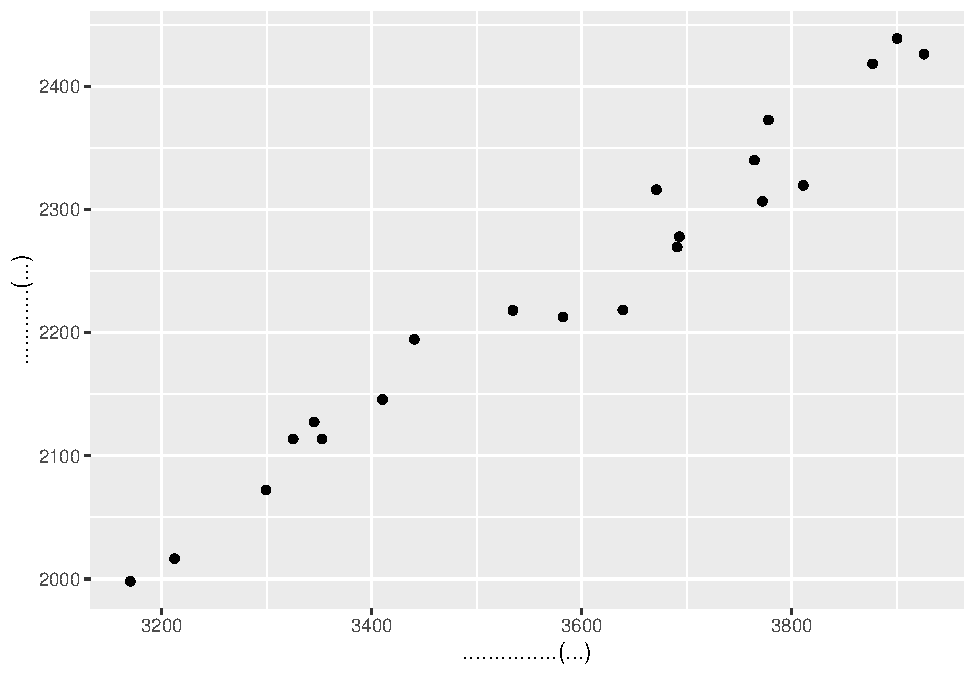
\includegraphics{_main_files/figure-latex/unnamed-chunk-14-1.pdf}

\hypertarget{ux7df4ux7fd2ux554fux984c-4-1-ux78baux8a8d}{%
\section*{練習問題 4-1 {[}確認{]}}\label{ux7df4ux7fd2ux554fux984c-4-1-ux78baux8a8d}}
\addcontentsline{toc}{section}{練習問題 4-1 {[}確認{]}}

\hypertarget{ux7df4ux7fd2ux554fux984c-4-2-ux5b9fux8a3c}{%
\section*{練習問題 4-2 {[}実証{]}}\label{ux7df4ux7fd2ux554fux984c-4-2-ux5b9fux8a3c}}
\addcontentsline{toc}{section}{練習問題 4-2 {[}実証{]}}

\begin{enumerate}
\def\labelenumi{(\arabic{enumi})}
\tightlist
\item
  データを読み込み, 回帰分析を実行する.
  Excelファイルの読み込みには\texttt{openxlsx::read.xlsx()}を用いる.
  列名が日本語だと扱いづらいため, これを変更しておく.
  \(gdp2013\_ln = \beta_0 + \beta_1 pop2013\_ln\)というモデルを立てると, \(\hat{\beta_0} = 7.623, \hat{\beta_1} = 1.075\)と求められる.
\end{enumerate}

\begin{Shaded}
\begin{Highlighting}[]
\NormalTok{data42 }\OtherTok{\textless{}{-}} \FunctionTok{read.xlsx}\NormalTok{(}\StringTok{"data/04\_第4章/data for chap 4 exercise 2.xlsx"}\NormalTok{)}
\FunctionTok{colnames}\NormalTok{(data42) }\OtherTok{\textless{}{-}} \FunctionTok{c}\NormalTok{(}\StringTok{"pref"}\NormalTok{, }\StringTok{"pop2013"}\NormalTok{, }\StringTok{"gdp2013"}\NormalTok{, }\StringTok{"pop2013\_ln"}\NormalTok{, }\StringTok{"gdp2013\_ln"}\NormalTok{)}

\NormalTok{model }\OtherTok{\textless{}{-}} \FunctionTok{lm}\NormalTok{(gdp2013\_ln }\SpecialCharTok{\textasciitilde{}}\NormalTok{ pop2013\_ln, }\AttributeTok{data =}\NormalTok{ data42)}
\NormalTok{model}
\DocumentationTok{\#\# }
\DocumentationTok{\#\# Call:}
\DocumentationTok{\#\# lm(formula = gdp2013\_ln \textasciitilde{} pop2013\_ln, data = data42)}
\DocumentationTok{\#\# }
\DocumentationTok{\#\# Coefficients:}
\DocumentationTok{\#\# (Intercept)   pop2013\_ln  }
\DocumentationTok{\#\#       7.623        1.075}
\end{Highlighting}
\end{Shaded}

\begin{enumerate}
\def\labelenumi{(\arabic{enumi})}
\setcounter{enumi}{1}
\tightlist
\item
  帰無仮説\(H_0\): \(\beta_1 = 1\)に関して, 統計量\(t = \frac{\hat{\beta_1} - \beta_1}{\text{SE}(\hat{\beta_1})} = 2.62773\)が求められる.
  これは自由度\(n-2 = 45\)で, 有意水準5\%のt検定の棄却域\((\infty, -2.014103]\), \([2.014103, \infty)\)に入っていることから帰無仮説は棄却される.
\end{enumerate}

\begin{Shaded}
\begin{Highlighting}[]
\NormalTok{beta1 }\OtherTok{\textless{}{-}}\NormalTok{ model}\SpecialCharTok{$}\NormalTok{coefficients[}\DecValTok{2}\NormalTok{]}
\NormalTok{sebeta1 }\OtherTok{\textless{}{-}} \FunctionTok{summary}\NormalTok{(model)}\SpecialCharTok{$}\NormalTok{coefficients[}\DecValTok{2}\NormalTok{, }\DecValTok{2}\NormalTok{]}
\NormalTok{n }\OtherTok{\textless{}{-}} \FunctionTok{dim}\NormalTok{(data42)[}\DecValTok{1}\NormalTok{]}

\NormalTok{t }\OtherTok{\textless{}{-}}\NormalTok{ (beta1 }\SpecialCharTok{{-}} \DecValTok{1}\NormalTok{)}\SpecialCharTok{/}\NormalTok{sebeta1}
\NormalTok{t}
\DocumentationTok{\#\# pop2013\_ln }
\DocumentationTok{\#\#    2.62773}
\FunctionTok{qt}\NormalTok{(}\FloatTok{0.975}\NormalTok{, n}\DecValTok{{-}2}\NormalTok{) }\CommentTok{\# 2.014103}
\DocumentationTok{\#\# [1] 2.014103}
\end{Highlighting}
\end{Shaded}

\begin{enumerate}
\def\labelenumi{(\arabic{enumi})}
\setcounter{enumi}{2}
\tightlist
\item
  \texttt{confint()}関数を用いると直接求められる.
\end{enumerate}

\begin{Shaded}
\begin{Highlighting}[]
\FunctionTok{confint}\NormalTok{(model, }\StringTok{\textquotesingle{}(Intercept)\textquotesingle{}}\NormalTok{, }\AttributeTok{level=}\FloatTok{0.90}\NormalTok{)}
\DocumentationTok{\#\#                  5 \%     95 \%}
\DocumentationTok{\#\# (Intercept) 7.257252 7.988132}
\end{Highlighting}
\end{Shaded}

\begin{enumerate}
\def\labelenumi{(\arabic{enumi})}
\setcounter{enumi}{3}
\item
  人口が1\%変化すると, GDPは\(\beta_1 = 1.075\)\%変化する.
\item
  \(\text{Var}(u) = \frac{\sum_{i=1}^n \hat{u}_i^2}{n-2} = 0.02245859\)と求められる.
  ln(人口)の分散は\texttt{var()}関数を用いると, 0.5964525と求められる.
\end{enumerate}

\begin{Shaded}
\begin{Highlighting}[]
\FunctionTok{sum}\NormalTok{(model}\SpecialCharTok{$}\NormalTok{residuals}\SpecialCharTok{\^{}}\DecValTok{2}\NormalTok{)}\SpecialCharTok{/}\NormalTok{(n}\DecValTok{{-}2}\NormalTok{)}
\DocumentationTok{\#\# [1] 0.02245859}

\NormalTok{var\_pop2013\_ln }\OtherTok{\textless{}{-}} \FunctionTok{var}\NormalTok{(data42}\SpecialCharTok{$}\NormalTok{pop2013\_ln)}
\NormalTok{var\_pop2013\_ln}
\DocumentationTok{\#\# [1] 0.5964525}
\end{Highlighting}
\end{Shaded}

\hypertarget{ux7df4ux7fd2ux554fux984c-4-3-ux78baux8a8d}{%
\section*{練習問題 4-3 {[}確認{]}}\label{ux7df4ux7fd2ux554fux984c-4-3-ux78baux8a8d}}
\addcontentsline{toc}{section}{練習問題 4-3 {[}確認{]}}

\hypertarget{ux7df4ux7fd2ux554fux984c-4-4-ux78baux8a8d}{%
\section*{練習問題 4-4 {[}確認{]}}\label{ux7df4ux7fd2ux554fux984c-4-4-ux78baux8a8d}}
\addcontentsline{toc}{section}{練習問題 4-4 {[}確認{]}}

\hypertarget{ux7df4ux7fd2ux554fux984c-4-5-ux78baux8a8d}{%
\section*{練習問題 4-5 {[}確認{]}}\label{ux7df4ux7fd2ux554fux984c-4-5-ux78baux8a8d}}
\addcontentsline{toc}{section}{練習問題 4-5 {[}確認{]}}

\hypertarget{ux7df4ux7fd2ux554fux984c-4-6-ux78baux8a8d}{%
\section*{練習問題 4-6 {[}確認{]}}\label{ux7df4ux7fd2ux554fux984c-4-6-ux78baux8a8d}}
\addcontentsline{toc}{section}{練習問題 4-6 {[}確認{]}}

\hypertarget{ux7df4ux7fd2ux554fux984c-4-7-ux78baux8a8d}{%
\section*{練習問題 4-7 {[}確認{]}}\label{ux7df4ux7fd2ux554fux984c-4-7-ux78baux8a8d}}
\addcontentsline{toc}{section}{練習問題 4-7 {[}確認{]}}

\hypertarget{ux7df4ux7fd2ux554fux984c-4-8-ux767aux5c55}{%
\section*{練習問題 4-8 {[}発展{]}}\label{ux7df4ux7fd2ux554fux984c-4-8-ux767aux5c55}}
\addcontentsline{toc}{section}{練習問題 4-8 {[}発展{]}}

\hypertarget{ux7df4ux7fd2ux554fux984c-4-9-ux767aux5c55}{%
\section*{練習問題 4-9 {[}発展{]}}\label{ux7df4ux7fd2ux554fux984c-4-9-ux767aux5c55}}
\addcontentsline{toc}{section}{練習問題 4-9 {[}発展{]}}

\hypertarget{ux7df4ux7fd2ux554fux984c-4-10-ux5b9fux8a3c}{%
\section*{練習問題 4-10 {[}実証{]}}\label{ux7df4ux7fd2ux554fux984c-4-10-ux5b9fux8a3c}}
\addcontentsline{toc}{section}{練習問題 4-10 {[}実証{]}}

\hypertarget{ch5}{%
\chapter*{第5章 重回帰モデルの推定と検定}\label{ch5}}
\addcontentsline{toc}{chapter}{第5章 重回帰モデルの推定と検定}

先に\href{https://www.yuhikaku.co.jp/books/detail/9784641053854}{出版社サイト}よりデータをダウンロードする.

\begin{Shaded}
\begin{Highlighting}[]
\CommentTok{\# サポートファイルへのリンク}
\NormalTok{curl }\OtherTok{\textless{}{-}} \StringTok{"https://www.yuhikaku.co.jp/static\_files/05385\_support05.zip"}
\CommentTok{\# ダウンロード保存用フォルダが存在しない場合, 作成}
\ControlFlowTok{if}\NormalTok{(}\SpecialCharTok{!}\FunctionTok{dir.exists}\NormalTok{(}\StringTok{"downloads"}\NormalTok{))\{}
    \FunctionTok{dir.create}\NormalTok{(}\StringTok{"downloads"}\NormalTok{)}
\NormalTok{\}}
\NormalTok{cdestfile }\OtherTok{\textless{}{-}} \StringTok{"downloads/support05.zip"}
\FunctionTok{download.file}\NormalTok{(curl, cdestfile)}
\CommentTok{\# データ保存用フォルダが存在しない場合, 作成}
\ControlFlowTok{if}\NormalTok{(}\SpecialCharTok{!}\FunctionTok{dir.exists}\NormalTok{(}\StringTok{"data"}\NormalTok{))\{}
    \FunctionTok{dir.create}\NormalTok{(}\StringTok{"data"}\NormalTok{)}
\NormalTok{\}}
\CommentTok{\# WSL上のRで解凍すると文字化けするので、Linuxのコマンドを外部呼び出し}
\CommentTok{\# Windowsの場合は別途コマンドを用いる.}
\ControlFlowTok{if}\NormalTok{(.Platform}\SpecialCharTok{$}\NormalTok{OS.type }\SpecialCharTok{==} \StringTok{"unix"}\NormalTok{) \{}
    \FunctionTok{system}\NormalTok{(}\FunctionTok{sprintf}\NormalTok{(}\StringTok{\textquotesingle{}unzip {-}n {-}Ocp932 \%s {-}d \%s\textquotesingle{}}\NormalTok{, }\StringTok{"downloads/support05.zip"}\NormalTok{, }\StringTok{"./data"}\NormalTok{))}
\NormalTok{\} }\ControlFlowTok{else}\NormalTok{ \{}
    \FunctionTok{print}\NormalTok{(}\StringTok{"Windowsで解凍するコマンドを別途追加せよ."}\NormalTok{)}
\NormalTok{\}}
\end{Highlighting}
\end{Shaded}

必要なライブラリを読み込む.

\begin{Shaded}
\begin{Highlighting}[]
\FunctionTok{library}\NormalTok{(tidyverse)}
\end{Highlighting}
\end{Shaded}

\hypertarget{ux7df4ux7fd2ux554fux984c-5-1-ux78baux8a8d}{%
\section*{練習問題 5-1 {[}確認{]}}\label{ux7df4ux7fd2ux554fux984c-5-1-ux78baux8a8d}}
\addcontentsline{toc}{section}{練習問題 5-1 {[}確認{]}}

\hypertarget{ux7df4ux7fd2ux554fux984c-5-2-ux78baux8a8d}{%
\section*{練習問題 5-2 {[}確認{]}}\label{ux7df4ux7fd2ux554fux984c-5-2-ux78baux8a8d}}
\addcontentsline{toc}{section}{練習問題 5-2 {[}確認{]}}

\hypertarget{ux7df4ux7fd2ux554fux984c-5-3-ux78baux8a8d}{%
\section*{練習問題 5-3 {[}確認{]}}\label{ux7df4ux7fd2ux554fux984c-5-3-ux78baux8a8d}}
\addcontentsline{toc}{section}{練習問題 5-3 {[}確認{]}}

\hypertarget{ux7df4ux7fd2ux554fux984c-5-4-ux78baux8a8d}{%
\section*{練習問題 5-4 {[}確認{]}}\label{ux7df4ux7fd2ux554fux984c-5-4-ux78baux8a8d}}
\addcontentsline{toc}{section}{練習問題 5-4 {[}確認{]}}

\hypertarget{ux7df4ux7fd2ux554fux984c-5-5-ux78baux8a8d}{%
\section*{練習問題 5-5 {[}確認{]}}\label{ux7df4ux7fd2ux554fux984c-5-5-ux78baux8a8d}}
\addcontentsline{toc}{section}{練習問題 5-5 {[}確認{]}}

\hypertarget{ux7df4ux7fd2ux554fux984c-5-6-ux78baux8a8d}{%
\section*{練習問題 5-6 {[}確認{]}}\label{ux7df4ux7fd2ux554fux984c-5-6-ux78baux8a8d}}
\addcontentsline{toc}{section}{練習問題 5-6 {[}確認{]}}

\hypertarget{ux7df4ux7fd2ux554fux984c-5-7-ux78baux8a8d}{%
\section*{練習問題 5-7 {[}確認{]}}\label{ux7df4ux7fd2ux554fux984c-5-7-ux78baux8a8d}}
\addcontentsline{toc}{section}{練習問題 5-7 {[}確認{]}}

\hypertarget{ux7df4ux7fd2ux554fux984c-5-8-ux78baux8a8d}{%
\section*{練習問題 5-8 {[}確認{]}}\label{ux7df4ux7fd2ux554fux984c-5-8-ux78baux8a8d}}
\addcontentsline{toc}{section}{練習問題 5-8 {[}確認{]}}

\hypertarget{ux7df4ux7fd2ux554fux984c-5-9-ux78baux8a8d}{%
\section*{練習問題 5-9 {[}確認{]}}\label{ux7df4ux7fd2ux554fux984c-5-9-ux78baux8a8d}}
\addcontentsline{toc}{section}{練習問題 5-9 {[}確認{]}}

\hypertarget{ux7df4ux7fd2ux554fux984c-5-10-ux767aux5c55}{%
\section*{練習問題 5-10 {[}発展{]}}\label{ux7df4ux7fd2ux554fux984c-5-10-ux767aux5c55}}
\addcontentsline{toc}{section}{練習問題 5-10 {[}発展{]}}

\hypertarget{ux7df4ux7fd2ux554fux984c-5-11-ux767aux5c55}{%
\section*{練習問題 5-11 {[}発展{]}}\label{ux7df4ux7fd2ux554fux984c-5-11-ux767aux5c55}}
\addcontentsline{toc}{section}{練習問題 5-11 {[}発展{]}}

\hypertarget{ux7df4ux7fd2ux554fux984c-5-12-ux767aux5c55}{%
\section*{練習問題 5-12 {[}発展{]}}\label{ux7df4ux7fd2ux554fux984c-5-12-ux767aux5c55}}
\addcontentsline{toc}{section}{練習問題 5-12 {[}発展{]}}

\hypertarget{ux7df4ux7fd2ux554fux984c-5-13-ux767aux5c55}{%
\section*{練習問題 5-13 {[}*発展{]}}\label{ux7df4ux7fd2ux554fux984c-5-13-ux767aux5c55}}
\addcontentsline{toc}{section}{練習問題 5-13 {[}*発展{]}}

\hypertarget{ux7df4ux7fd2ux554fux984c-5-14-ux5b9fux8a3c}{%
\section*{練習問題 5-14 {[}実証{]}}\label{ux7df4ux7fd2ux554fux984c-5-14-ux5b9fux8a3c}}
\addcontentsline{toc}{section}{練習問題 5-14 {[}実証{]}}

\hypertarget{ux7df4ux7fd2ux554fux984c-5-15-ux5b9fux8a3c}{%
\section*{練習問題 5-15 {[}実証{]}}\label{ux7df4ux7fd2ux554fux984c-5-15-ux5b9fux8a3c}}
\addcontentsline{toc}{section}{練習問題 5-15 {[}実証{]}}

\hypertarget{ch6}{%
\chapter*{第6章 パネルデータ分析}\label{ch6}}
\addcontentsline{toc}{chapter}{第6章 パネルデータ分析}

先に\href{https://www.yuhikaku.co.jp/books/detail/9784641053854}{出版社サイト}よりデータをダウンロードする.

\begin{Shaded}
\begin{Highlighting}[]
\CommentTok{\# サポートファイルへのリンク}
\NormalTok{curl }\OtherTok{\textless{}{-}} \StringTok{"https://www.yuhikaku.co.jp/static\_files/05385\_support06.zip"}
\CommentTok{\# ダウンロード保存用フォルダが存在しない場合, 作成}
\ControlFlowTok{if}\NormalTok{(}\SpecialCharTok{!}\FunctionTok{dir.exists}\NormalTok{(}\StringTok{"downloads"}\NormalTok{))\{}
    \FunctionTok{dir.create}\NormalTok{(}\StringTok{"downloads"}\NormalTok{)}
\NormalTok{\}}
\NormalTok{cdestfile }\OtherTok{\textless{}{-}} \StringTok{"downloads/support06.zip"}
\FunctionTok{download.file}\NormalTok{(curl, cdestfile)}
\CommentTok{\# データ保存用フォルダが存在しない場合, 作成}
\ControlFlowTok{if}\NormalTok{(}\SpecialCharTok{!}\FunctionTok{dir.exists}\NormalTok{(}\StringTok{"data"}\NormalTok{))\{}
    \FunctionTok{dir.create}\NormalTok{(}\StringTok{"data"}\NormalTok{)}
\NormalTok{\}}
\CommentTok{\# WSL上のRで解凍すると文字化けするので、Linuxのコマンドを外部呼び出し}
\CommentTok{\# Windowsの場合は別途コマンドを用いる.}
\ControlFlowTok{if}\NormalTok{(.Platform}\SpecialCharTok{$}\NormalTok{OS.type }\SpecialCharTok{==} \StringTok{"unix"}\NormalTok{) \{}
    \FunctionTok{system}\NormalTok{(}\FunctionTok{sprintf}\NormalTok{(}\StringTok{\textquotesingle{}unzip {-}n {-}Ocp932 \%s {-}d \%s\textquotesingle{}}\NormalTok{, }\StringTok{"downloads/support06.zip"}\NormalTok{, }\StringTok{"./data"}\NormalTok{))}
\NormalTok{\} }\ControlFlowTok{else}\NormalTok{ \{}
    \FunctionTok{print}\NormalTok{(}\StringTok{"Windowsで解凍するコマンドを別途追加せよ."}\NormalTok{)}
\NormalTok{\}}
\end{Highlighting}
\end{Shaded}

\hypertarget{ux7df4ux7fd2ux554fux984c-6-1-ux78baux8a8d}{%
\section*{練習問題 6-1 {[}確認{]}}\label{ux7df4ux7fd2ux554fux984c-6-1-ux78baux8a8d}}
\addcontentsline{toc}{section}{練習問題 6-1 {[}確認{]}}

\hypertarget{ux7df4ux7fd2ux554fux984c-6-2-ux78baux8a8d}{%
\section*{練習問題 6-2 {[}確認{]}}\label{ux7df4ux7fd2ux554fux984c-6-2-ux78baux8a8d}}
\addcontentsline{toc}{section}{練習問題 6-2 {[}確認{]}}

\hypertarget{ux7df4ux7fd2ux554fux984c-6-3-ux78baux8a8d}{%
\section*{練習問題 6-3 {[}確認{]}}\label{ux7df4ux7fd2ux554fux984c-6-3-ux78baux8a8d}}
\addcontentsline{toc}{section}{練習問題 6-3 {[}確認{]}}

\hypertarget{ux7df4ux7fd2ux554fux984c-6-4-ux78baux8a8d}{%
\section*{練習問題 6-4 {[}確認{]}}\label{ux7df4ux7fd2ux554fux984c-6-4-ux78baux8a8d}}
\addcontentsline{toc}{section}{練習問題 6-4 {[}確認{]}}

\hypertarget{ux7df4ux7fd2ux554fux984c-6-5-ux78baux8a8d}{%
\section*{練習問題 6-5 {[}確認{]}}\label{ux7df4ux7fd2ux554fux984c-6-5-ux78baux8a8d}}
\addcontentsline{toc}{section}{練習問題 6-5 {[}確認{]}}

\hypertarget{ux7df4ux7fd2ux554fux984c-6-6-ux78baux8a8d}{%
\section*{練習問題 6-6 {[}確認{]}}\label{ux7df4ux7fd2ux554fux984c-6-6-ux78baux8a8d}}
\addcontentsline{toc}{section}{練習問題 6-6 {[}確認{]}}

\hypertarget{ux7df4ux7fd2ux554fux984c-6-7-ux78baux8a8d}{%
\section*{練習問題 6-7 {[}確認{]}}\label{ux7df4ux7fd2ux554fux984c-6-7-ux78baux8a8d}}
\addcontentsline{toc}{section}{練習問題 6-7 {[}確認{]}}

\hypertarget{ux7df4ux7fd2ux554fux984c-6-8-ux767aux5c55}{%
\section*{練習問題 6-8 {[}発展{]}}\label{ux7df4ux7fd2ux554fux984c-6-8-ux767aux5c55}}
\addcontentsline{toc}{section}{練習問題 6-8 {[}発展{]}}

\hypertarget{ux7df4ux7fd2ux554fux984c-6-9-ux767aux5c55}{%
\section*{練習問題 6-9 {[}発展{]}}\label{ux7df4ux7fd2ux554fux984c-6-9-ux767aux5c55}}
\addcontentsline{toc}{section}{練習問題 6-9 {[}発展{]}}

\hypertarget{ux7df4ux7fd2ux554fux984c-6-10-ux5b9fux8a3c}{%
\section*{練習問題 6-10 {[}実証{]}}\label{ux7df4ux7fd2ux554fux984c-6-10-ux5b9fux8a3c}}
\addcontentsline{toc}{section}{練習問題 6-10 {[}実証{]}}

\hypertarget{ux7df4ux7fd2ux554fux984c-6-11-ux5b9fux8a3c}{%
\section*{練習問題 6-11 {[}実証{]}}\label{ux7df4ux7fd2ux554fux984c-6-11-ux5b9fux8a3c}}
\addcontentsline{toc}{section}{練習問題 6-11 {[}実証{]}}

\hypertarget{ch7}{%
\chapter*{第7章 操作変数法}\label{ch7}}
\addcontentsline{toc}{chapter}{第7章 操作変数法}

先に\href{https://www.yuhikaku.co.jp/books/detail/9784641053854}{出版社サイト}よりデータをダウンロードする.

\begin{Shaded}
\begin{Highlighting}[]
\CommentTok{\# サポートファイルへのリンク}
\NormalTok{curl }\OtherTok{\textless{}{-}} \StringTok{"https://www.yuhikaku.co.jp/static\_files/05385\_support07.zip"}
\CommentTok{\# ダウンロード保存用フォルダが存在しない場合, 作成}
\ControlFlowTok{if}\NormalTok{(}\SpecialCharTok{!}\FunctionTok{dir.exists}\NormalTok{(}\StringTok{"downloads"}\NormalTok{))\{}
    \FunctionTok{dir.create}\NormalTok{(}\StringTok{"downloads"}\NormalTok{)}
\NormalTok{\}}
\NormalTok{cdestfile }\OtherTok{\textless{}{-}} \StringTok{"downloads/support07.zip"}
\FunctionTok{download.file}\NormalTok{(curl, cdestfile)}
\CommentTok{\# データ保存用フォルダが存在しない場合, 作成}
\ControlFlowTok{if}\NormalTok{(}\SpecialCharTok{!}\FunctionTok{dir.exists}\NormalTok{(}\StringTok{"data"}\NormalTok{))\{}
    \FunctionTok{dir.create}\NormalTok{(}\StringTok{"data"}\NormalTok{)}
\NormalTok{\}}
\CommentTok{\# WSL上のRで解凍すると文字化けするので、Linuxのコマンドを外部呼び出し}
\CommentTok{\# Windowsの場合は別途コマンドを用いる.}
\ControlFlowTok{if}\NormalTok{(.Platform}\SpecialCharTok{$}\NormalTok{OS.type }\SpecialCharTok{==} \StringTok{"unix"}\NormalTok{) \{}
    \FunctionTok{system}\NormalTok{(}\FunctionTok{sprintf}\NormalTok{(}\StringTok{\textquotesingle{}unzip {-}n {-}Ocp932 \%s {-}d \%s\textquotesingle{}}\NormalTok{, }\StringTok{"downloads/support07.zip"}\NormalTok{, }\StringTok{"./data"}\NormalTok{))}
\NormalTok{\} }\ControlFlowTok{else}\NormalTok{ \{}
    \FunctionTok{print}\NormalTok{(}\StringTok{"Windowsで解凍するコマンドを別途追加せよ."}\NormalTok{)}
\NormalTok{\}}
\end{Highlighting}
\end{Shaded}

\hypertarget{ux7df4ux7fd2ux554fux984c-7-1-ux78baux8a8d}{%
\section*{練習問題 7-1 {[}確認{]}}\label{ux7df4ux7fd2ux554fux984c-7-1-ux78baux8a8d}}
\addcontentsline{toc}{section}{練習問題 7-1 {[}確認{]}}

\hypertarget{ux7df4ux7fd2ux554fux984c-7-2-ux78baux8a8d}{%
\section*{練習問題 7-2 {[}確認{]}}\label{ux7df4ux7fd2ux554fux984c-7-2-ux78baux8a8d}}
\addcontentsline{toc}{section}{練習問題 7-2 {[}確認{]}}

\hypertarget{ux7df4ux7fd2ux554fux984c-7-3-ux78baux8a8d}{%
\section*{練習問題 7-3 {[}確認{]}}\label{ux7df4ux7fd2ux554fux984c-7-3-ux78baux8a8d}}
\addcontentsline{toc}{section}{練習問題 7-3 {[}確認{]}}

\hypertarget{ux7df4ux7fd2ux554fux984c-7-4-ux78baux8a8d}{%
\section*{練習問題 7-4 {[}確認{]}}\label{ux7df4ux7fd2ux554fux984c-7-4-ux78baux8a8d}}
\addcontentsline{toc}{section}{練習問題 7-4 {[}確認{]}}

\hypertarget{ux7df4ux7fd2ux554fux984c-7-5-ux78baux8a8d}{%
\section*{練習問題 7-5 {[}確認{]}}\label{ux7df4ux7fd2ux554fux984c-7-5-ux78baux8a8d}}
\addcontentsline{toc}{section}{練習問題 7-5 {[}確認{]}}

\hypertarget{ux7df4ux7fd2ux554fux984c-7-6-ux78baux8a8d}{%
\section*{練習問題 7-6 {[}確認{]}}\label{ux7df4ux7fd2ux554fux984c-7-6-ux78baux8a8d}}
\addcontentsline{toc}{section}{練習問題 7-6 {[}確認{]}}

\hypertarget{ux7df4ux7fd2ux554fux984c-7-7-ux78baux8a8d}{%
\section*{練習問題 7-7 {[}確認{]}}\label{ux7df4ux7fd2ux554fux984c-7-7-ux78baux8a8d}}
\addcontentsline{toc}{section}{練習問題 7-7 {[}確認{]}}

\hypertarget{ux7df4ux7fd2ux554fux984c-7-8-ux78baux8a8d}{%
\section*{練習問題 7-8 {[}確認{]}}\label{ux7df4ux7fd2ux554fux984c-7-8-ux78baux8a8d}}
\addcontentsline{toc}{section}{練習問題 7-8 {[}確認{]}}

\hypertarget{ux7df4ux7fd2ux554fux984c-7-9-ux78baux8a8d}{%
\section*{練習問題 7-9 {[}確認{]}}\label{ux7df4ux7fd2ux554fux984c-7-9-ux78baux8a8d}}
\addcontentsline{toc}{section}{練習問題 7-9 {[}確認{]}}

\hypertarget{ux7df4ux7fd2ux554fux984c-7-10-ux78baux8a8d}{%
\section*{練習問題 7-10 {[}確認{]}}\label{ux7df4ux7fd2ux554fux984c-7-10-ux78baux8a8d}}
\addcontentsline{toc}{section}{練習問題 7-10 {[}確認{]}}

\hypertarget{ux7df4ux7fd2ux554fux984c-7-11-ux767aux5c55}{%
\section*{練習問題 7-11 {[}発展{]}}\label{ux7df4ux7fd2ux554fux984c-7-11-ux767aux5c55}}
\addcontentsline{toc}{section}{練習問題 7-11 {[}発展{]}}

\hypertarget{ux7df4ux7fd2ux554fux984c-7-12-ux767aux5c55}{%
\section*{練習問題 7-12 {[}発展{]}}\label{ux7df4ux7fd2ux554fux984c-7-12-ux767aux5c55}}
\addcontentsline{toc}{section}{練習問題 7-12 {[}発展{]}}

\hypertarget{ux7df4ux7fd2ux554fux984c-7-13-ux5b9fux8a3c}{%
\section*{練習問題 7-13 {[}実証{]}}\label{ux7df4ux7fd2ux554fux984c-7-13-ux5b9fux8a3c}}
\addcontentsline{toc}{section}{練習問題 7-13 {[}実証{]}}

\hypertarget{ch8}{%
\chapter*{第8章 制限従属変数モデル}\label{ch8}}
\addcontentsline{toc}{chapter}{第8章 制限従属変数モデル}

先に\href{https://www.yuhikaku.co.jp/books/detail/9784641053854}{出版社サイト}よりデータをダウンロードする.

\begin{Shaded}
\begin{Highlighting}[]
\CommentTok{\# サポートファイルへのリンク}
\NormalTok{curl }\OtherTok{\textless{}{-}} \StringTok{"https://www.yuhikaku.co.jp/static\_files/05385\_support08.zip"}
\CommentTok{\# ダウンロード保存用フォルダが存在しない場合, 作成}
\ControlFlowTok{if}\NormalTok{(}\SpecialCharTok{!}\FunctionTok{dir.exists}\NormalTok{(}\StringTok{"downloads"}\NormalTok{))\{}
    \FunctionTok{dir.create}\NormalTok{(}\StringTok{"downloads"}\NormalTok{)}
\NormalTok{\}}
\NormalTok{cdestfile }\OtherTok{\textless{}{-}} \StringTok{"downloads/support08.zip"}
\FunctionTok{download.file}\NormalTok{(curl, cdestfile)}
\CommentTok{\# データ保存用フォルダが存在しない場合, 作成}
\ControlFlowTok{if}\NormalTok{(}\SpecialCharTok{!}\FunctionTok{dir.exists}\NormalTok{(}\StringTok{"data"}\NormalTok{))\{}
    \FunctionTok{dir.create}\NormalTok{(}\StringTok{"data"}\NormalTok{)}
\NormalTok{\}}
\CommentTok{\# WSL上のRで解凍すると文字化けするので、Linuxのコマンドを外部呼び出し}
\CommentTok{\# Windowsの場合は別途コマンドを用いる.}
\ControlFlowTok{if}\NormalTok{(.Platform}\SpecialCharTok{$}\NormalTok{OS.type }\SpecialCharTok{==} \StringTok{"unix"}\NormalTok{) \{}
    \FunctionTok{system}\NormalTok{(}\FunctionTok{sprintf}\NormalTok{(}\StringTok{\textquotesingle{}unzip {-}n {-}Ocp932 \%s {-}d \%s\textquotesingle{}}\NormalTok{, }\StringTok{"downloads/support08.zip"}\NormalTok{, }\StringTok{"./data"}\NormalTok{))}
\NormalTok{\} }\ControlFlowTok{else}\NormalTok{ \{}
    \FunctionTok{print}\NormalTok{(}\StringTok{"Windowsで解凍するコマンドを別途追加せよ."}\NormalTok{)}
\NormalTok{\}}
\end{Highlighting}
\end{Shaded}

\hypertarget{ux7df4ux7fd2ux554fux984c-8-1-ux78baux8a8d}{%
\section*{練習問題 8-1 {[}確認{]}}\label{ux7df4ux7fd2ux554fux984c-8-1-ux78baux8a8d}}
\addcontentsline{toc}{section}{練習問題 8-1 {[}確認{]}}

\hypertarget{ux7df4ux7fd2ux554fux984c-8-2-ux78baux8a8d}{%
\section*{練習問題 8-2 {[}確認{]}}\label{ux7df4ux7fd2ux554fux984c-8-2-ux78baux8a8d}}
\addcontentsline{toc}{section}{練習問題 8-2 {[}確認{]}}

\hypertarget{ux7df4ux7fd2ux554fux984c-8-3-ux767aux5c55}{%
\section*{練習問題 8-3 {[}発展{]}}\label{ux7df4ux7fd2ux554fux984c-8-3-ux767aux5c55}}
\addcontentsline{toc}{section}{練習問題 8-3 {[}発展{]}}

\hypertarget{ux7df4ux7fd2ux554fux984c-8-4-ux5b9fux8a3c}{%
\section*{練習問題 8-4 {[}実証{]}}\label{ux7df4ux7fd2ux554fux984c-8-4-ux5b9fux8a3c}}
\addcontentsline{toc}{section}{練習問題 8-4 {[}実証{]}}

\hypertarget{ch9}{%
\chapter*{第9章 政策評価モデル}\label{ch9}}
\addcontentsline{toc}{chapter}{第9章 政策評価モデル}

先に\href{https://www.yuhikaku.co.jp/books/detail/9784641053854}{出版社サイト}よりデータをダウンロードする.

\begin{Shaded}
\begin{Highlighting}[]
\CommentTok{\# サポートファイルへのリンク}
\NormalTok{curl }\OtherTok{\textless{}{-}} \StringTok{"https://www.yuhikaku.co.jp/static\_files/05385\_support09.zip"}
\CommentTok{\# ダウンロード保存用フォルダが存在しない場合, 作成}
\ControlFlowTok{if}\NormalTok{(}\SpecialCharTok{!}\FunctionTok{dir.exists}\NormalTok{(}\StringTok{"downloads"}\NormalTok{))\{}
    \FunctionTok{dir.create}\NormalTok{(}\StringTok{"downloads"}\NormalTok{)}
\NormalTok{\}}
\NormalTok{cdestfile }\OtherTok{\textless{}{-}} \StringTok{"downloads/support09.zip"}
\FunctionTok{download.file}\NormalTok{(curl, cdestfile)}
\CommentTok{\# データ保存用フォルダが存在しない場合, 作成}
\ControlFlowTok{if}\NormalTok{(}\SpecialCharTok{!}\FunctionTok{dir.exists}\NormalTok{(}\StringTok{"data"}\NormalTok{))\{}
    \FunctionTok{dir.create}\NormalTok{(}\StringTok{"data"}\NormalTok{)}
\NormalTok{\}}
\CommentTok{\# WSL上のRで解凍すると文字化けするので、Linuxのコマンドを外部呼び出し}
\CommentTok{\# Windowsの場合は別途コマンドを用いる.}
\ControlFlowTok{if}\NormalTok{(.Platform}\SpecialCharTok{$}\NormalTok{OS.type }\SpecialCharTok{==} \StringTok{"unix"}\NormalTok{) \{}
    \FunctionTok{system}\NormalTok{(}\FunctionTok{sprintf}\NormalTok{(}\StringTok{\textquotesingle{}unzip {-}n {-}Ocp932 \%s {-}d \%s\textquotesingle{}}\NormalTok{, }\StringTok{"downloads/support09.zip"}\NormalTok{, }\StringTok{"./data"}\NormalTok{))}
\NormalTok{\} }\ControlFlowTok{else}\NormalTok{ \{}
    \FunctionTok{print}\NormalTok{(}\StringTok{"Windowsで解凍するコマンドを別途追加せよ."}\NormalTok{)}
\NormalTok{\}}
\end{Highlighting}
\end{Shaded}

\hypertarget{ux7df4ux7fd2ux554fux984c-9-1-ux78baux8a8d}{%
\section*{練習問題 9-1 {[}確認{]}}\label{ux7df4ux7fd2ux554fux984c-9-1-ux78baux8a8d}}
\addcontentsline{toc}{section}{練習問題 9-1 {[}確認{]}}

\hypertarget{ux7df4ux7fd2ux554fux984c-9-2-ux78baux8a8d}{%
\section*{練習問題 9-2 {[}確認{]}}\label{ux7df4ux7fd2ux554fux984c-9-2-ux78baux8a8d}}
\addcontentsline{toc}{section}{練習問題 9-2 {[}確認{]}}

\hypertarget{ux7df4ux7fd2ux554fux984c-9-3-ux767aux5c55}{%
\section*{練習問題 9-3 {[}発展{]}}\label{ux7df4ux7fd2ux554fux984c-9-3-ux767aux5c55}}
\addcontentsline{toc}{section}{練習問題 9-3 {[}発展{]}}

\hypertarget{ux7df4ux7fd2ux554fux984c-9-4-ux767aux5c55}{%
\section*{練習問題 9-4 {[}発展{]}}\label{ux7df4ux7fd2ux554fux984c-9-4-ux767aux5c55}}
\addcontentsline{toc}{section}{練習問題 9-4 {[}発展{]}}

\hypertarget{ux7df4ux7fd2ux554fux984c-9-5-ux5b9fux8a3c}{%
\section*{練習問題 9-5 {[}実証{]}}\label{ux7df4ux7fd2ux554fux984c-9-5-ux5b9fux8a3c}}
\addcontentsline{toc}{section}{練習問題 9-5 {[}実証{]}}

\hypertarget{ch10}{%
\chapter*{第10章 系列相関と時系列モデル}\label{ch10}}
\addcontentsline{toc}{chapter}{第10章 系列相関と時系列モデル}

先に\href{https://www.yuhikaku.co.jp/books/detail/9784641053854}{出版社サイト}よりデータをダウンロードする.

\begin{Shaded}
\begin{Highlighting}[]
\CommentTok{\# サポートファイルへのリンク}
\NormalTok{curl }\OtherTok{\textless{}{-}} \StringTok{"https://www.yuhikaku.co.jp/static\_files/05385\_support10.zip"}
\CommentTok{\# ダウンロード保存用フォルダが存在しない場合, 作成}
\ControlFlowTok{if}\NormalTok{(}\SpecialCharTok{!}\FunctionTok{dir.exists}\NormalTok{(}\StringTok{"downloads"}\NormalTok{))\{}
    \FunctionTok{dir.create}\NormalTok{(}\StringTok{"downloads"}\NormalTok{)}
\NormalTok{\}}
\NormalTok{cdestfile }\OtherTok{\textless{}{-}} \StringTok{"downloads/support10.zip"}
\FunctionTok{download.file}\NormalTok{(curl, cdestfile)}
\CommentTok{\# データ保存用フォルダが存在しない場合, 作成}
\ControlFlowTok{if}\NormalTok{(}\SpecialCharTok{!}\FunctionTok{dir.exists}\NormalTok{(}\StringTok{"data"}\NormalTok{))\{}
    \FunctionTok{dir.create}\NormalTok{(}\StringTok{"data"}\NormalTok{)}
\NormalTok{\}}
\CommentTok{\# WSL上のRで解凍すると文字化けするので、Linuxのコマンドを外部呼び出し}
\CommentTok{\# Windowsの場合は別途コマンドを用いる.}
\ControlFlowTok{if}\NormalTok{(.Platform}\SpecialCharTok{$}\NormalTok{OS.type }\SpecialCharTok{==} \StringTok{"unix"}\NormalTok{) \{}
    \FunctionTok{system}\NormalTok{(}\FunctionTok{sprintf}\NormalTok{(}\StringTok{\textquotesingle{}unzip {-}n {-}Ocp932 \%s {-}d \%s\textquotesingle{}}\NormalTok{, }\StringTok{"downloads/support10.zip"}\NormalTok{, }\StringTok{"./data"}\NormalTok{))}
\NormalTok{\} }\ControlFlowTok{else}\NormalTok{ \{}
    \FunctionTok{print}\NormalTok{(}\StringTok{"Windowsで解凍するコマンドを別途追加せよ."}\NormalTok{)}
\NormalTok{\}}
\end{Highlighting}
\end{Shaded}

\hypertarget{ux7df4ux7fd2ux554fux984c-10-1-ux78baux8a8d}{%
\section*{練習問題 10-1 {[}確認{]}}\label{ux7df4ux7fd2ux554fux984c-10-1-ux78baux8a8d}}
\addcontentsline{toc}{section}{練習問題 10-1 {[}確認{]}}

\hypertarget{ux7df4ux7fd2ux554fux984c-10-2-ux78baux8a8d}{%
\section*{練習問題 10-2 {[}確認{]}}\label{ux7df4ux7fd2ux554fux984c-10-2-ux78baux8a8d}}
\addcontentsline{toc}{section}{練習問題 10-2 {[}確認{]}}

\hypertarget{ux7df4ux7fd2ux554fux984c-10-3-ux78baux8a8d}{%
\section*{練習問題 10-3 {[}確認{]}}\label{ux7df4ux7fd2ux554fux984c-10-3-ux78baux8a8d}}
\addcontentsline{toc}{section}{練習問題 10-3 {[}確認{]}}

\hypertarget{ux7df4ux7fd2ux554fux984c-10-4-ux78baux8a8d}{%
\section*{練習問題 10-4 {[}確認{]}}\label{ux7df4ux7fd2ux554fux984c-10-4-ux78baux8a8d}}
\addcontentsline{toc}{section}{練習問題 10-4 {[}確認{]}}

\hypertarget{ux7df4ux7fd2ux554fux984c-10-5-ux78baux8a8d}{%
\section*{練習問題 10-5 {[}確認{]}}\label{ux7df4ux7fd2ux554fux984c-10-5-ux78baux8a8d}}
\addcontentsline{toc}{section}{練習問題 10-5 {[}確認{]}}

\hypertarget{ux7df4ux7fd2ux554fux984c-10-6-ux78baux8a8d}{%
\section*{練習問題 10-6 {[}確認{]}}\label{ux7df4ux7fd2ux554fux984c-10-6-ux78baux8a8d}}
\addcontentsline{toc}{section}{練習問題 10-6 {[}確認{]}}

\hypertarget{ux7df4ux7fd2ux554fux984c-10-7-ux767aux5c55}{%
\section*{練習問題 10-7 {[}発展{]}}\label{ux7df4ux7fd2ux554fux984c-10-7-ux767aux5c55}}
\addcontentsline{toc}{section}{練習問題 10-7 {[}発展{]}}

\hypertarget{ux7df4ux7fd2ux554fux984c-10-8-ux767aux5c55}{%
\section*{練習問題 10-8 {[}発展{]}}\label{ux7df4ux7fd2ux554fux984c-10-8-ux767aux5c55}}
\addcontentsline{toc}{section}{練習問題 10-8 {[}発展{]}}

\hypertarget{ux7df4ux7fd2ux554fux984c-10-9-ux5b9fux8a3c}{%
\section*{練習問題 10-9 {[}実証{]}}\label{ux7df4ux7fd2ux554fux984c-10-9-ux5b9fux8a3c}}
\addcontentsline{toc}{section}{練習問題 10-9 {[}実証{]}}

\hypertarget{ux7df4ux7fd2ux554fux984c-10-10-ux5b9fux8a3c}{%
\section*{練習問題 10-10 {[}実証{]}}\label{ux7df4ux7fd2ux554fux984c-10-10-ux5b9fux8a3c}}
\addcontentsline{toc}{section}{練習問題 10-10 {[}実証{]}}

\hypertarget{ch11}{%
\chapter*{第11章 トレンドと構造変化}\label{ch11}}
\addcontentsline{toc}{chapter}{第11章 トレンドと構造変化}

先に\href{https://www.yuhikaku.co.jp/books/detail/9784641053854}{出版社サイト}よりデータをダウンロードする.

\begin{Shaded}
\begin{Highlighting}[]
\CommentTok{\# サポートファイルへのリンク}
\NormalTok{curl }\OtherTok{\textless{}{-}} \StringTok{"https://www.yuhikaku.co.jp/static\_files/05385\_support11.zip"}
\CommentTok{\# ダウンロード保存用フォルダが存在しない場合, 作成}
\ControlFlowTok{if}\NormalTok{(}\SpecialCharTok{!}\FunctionTok{dir.exists}\NormalTok{(}\StringTok{"downloads"}\NormalTok{))\{}
    \FunctionTok{dir.create}\NormalTok{(}\StringTok{"downloads"}\NormalTok{)}
\NormalTok{\}}
\NormalTok{cdestfile }\OtherTok{\textless{}{-}} \StringTok{"downloads/support11.zip"}
\FunctionTok{download.file}\NormalTok{(curl, cdestfile)}
\CommentTok{\# データ保存用フォルダが存在しない場合, 作成}
\ControlFlowTok{if}\NormalTok{(}\SpecialCharTok{!}\FunctionTok{dir.exists}\NormalTok{(}\StringTok{"data"}\NormalTok{))\{}
    \FunctionTok{dir.create}\NormalTok{(}\StringTok{"data"}\NormalTok{)}
\NormalTok{\}}
\CommentTok{\# WSL上のRで解凍すると文字化けするので、Linuxのコマンドを外部呼び出し}
\CommentTok{\# Windowsの場合は別途コマンドを用いる.}
\ControlFlowTok{if}\NormalTok{(.Platform}\SpecialCharTok{$}\NormalTok{OS.type }\SpecialCharTok{==} \StringTok{"unix"}\NormalTok{) \{}
    \FunctionTok{system}\NormalTok{(}\FunctionTok{sprintf}\NormalTok{(}\StringTok{\textquotesingle{}unzip {-}n {-}Ocp932 \%s {-}d \%s\textquotesingle{}}\NormalTok{, }\StringTok{"downloads/support11.zip"}\NormalTok{, }\StringTok{"./data"}\NormalTok{))}
\NormalTok{\} }\ControlFlowTok{else}\NormalTok{ \{}
    \FunctionTok{print}\NormalTok{(}\StringTok{"Windowsで解凍するコマンドを別途追加せよ."}\NormalTok{)}
\NormalTok{\}}
\end{Highlighting}
\end{Shaded}

\hypertarget{ux7df4ux7fd2ux554fux984c-11-1-ux78baux8a8d}{%
\section*{練習問題 11-1 {[}確認{]}}\label{ux7df4ux7fd2ux554fux984c-11-1-ux78baux8a8d}}
\addcontentsline{toc}{section}{練習問題 11-1 {[}確認{]}}

\hypertarget{ux7df4ux7fd2ux554fux984c-11-2-ux78baux8a8d}{%
\section*{練習問題 11-2 {[}確認{]}}\label{ux7df4ux7fd2ux554fux984c-11-2-ux78baux8a8d}}
\addcontentsline{toc}{section}{練習問題 11-2 {[}確認{]}}

\hypertarget{ux7df4ux7fd2ux554fux984c-11-3-ux78baux8a8d}{%
\section*{練習問題 11-3 {[}確認{]}}\label{ux7df4ux7fd2ux554fux984c-11-3-ux78baux8a8d}}
\addcontentsline{toc}{section}{練習問題 11-3 {[}確認{]}}

\hypertarget{ux7df4ux7fd2ux554fux984c-11-4-ux78baux8a8d}{%
\section*{練習問題 11-4 {[}確認{]}}\label{ux7df4ux7fd2ux554fux984c-11-4-ux78baux8a8d}}
\addcontentsline{toc}{section}{練習問題 11-4 {[}確認{]}}

\hypertarget{ux7df4ux7fd2ux554fux984c-11-5-ux78baux8a8d}{%
\section*{練習問題 11-5 {[}確認{]}}\label{ux7df4ux7fd2ux554fux984c-11-5-ux78baux8a8d}}
\addcontentsline{toc}{section}{練習問題 11-5 {[}確認{]}}

\hypertarget{ux7df4ux7fd2ux554fux984c-11-6-ux767aux5c55}{%
\section*{練習問題 11-6 {[}発展{]}}\label{ux7df4ux7fd2ux554fux984c-11-6-ux767aux5c55}}
\addcontentsline{toc}{section}{練習問題 11-6 {[}発展{]}}

\hypertarget{ux7df4ux7fd2ux554fux984c-11-7-ux767aux5c55}{%
\section*{練習問題 11-7 {[}発展{]}}\label{ux7df4ux7fd2ux554fux984c-11-7-ux767aux5c55}}
\addcontentsline{toc}{section}{練習問題 11-7 {[}発展{]}}

\hypertarget{ux7df4ux7fd2ux554fux984c-11-8-ux5b9fux8a3c}{%
\section*{練習問題 11-8 {[}実証{]}}\label{ux7df4ux7fd2ux554fux984c-11-8-ux5b9fux8a3c}}
\addcontentsline{toc}{section}{練習問題 11-8 {[}実証{]}}

\hypertarget{ux7df4ux7fd2ux554fux984c-11-9-ux5b9fux8a3c}{%
\section*{練習問題 11-9 {[}実証{]}}\label{ux7df4ux7fd2ux554fux984c-11-9-ux5b9fux8a3c}}
\addcontentsline{toc}{section}{練習問題 11-9 {[}実証{]}}

\hypertarget{ch12}{%
\chapter*{第12章 VARモデル}\label{ch12}}
\addcontentsline{toc}{chapter}{第12章 VARモデル}

先に\href{https://www.yuhikaku.co.jp/books/detail/9784641053854}{出版社サイト}よりデータをダウンロードする.

\begin{Shaded}
\begin{Highlighting}[]
\CommentTok{\# サポートファイルへのリンク}
\NormalTok{curl }\OtherTok{\textless{}{-}} \StringTok{"https://www.yuhikaku.co.jp/static\_files/05385\_support12.zip"}
\CommentTok{\# ダウンロード保存用フォルダが存在しない場合, 作成}
\ControlFlowTok{if}\NormalTok{(}\SpecialCharTok{!}\FunctionTok{dir.exists}\NormalTok{(}\StringTok{"downloads"}\NormalTok{))\{}
    \FunctionTok{dir.create}\NormalTok{(}\StringTok{"downloads"}\NormalTok{)}
\NormalTok{\}}
\NormalTok{cdestfile }\OtherTok{\textless{}{-}} \StringTok{"downloads/support12.zip"}
\FunctionTok{download.file}\NormalTok{(curl, cdestfile)}
\CommentTok{\# データ保存用フォルダが存在しない場合, 作成}
\ControlFlowTok{if}\NormalTok{(}\SpecialCharTok{!}\FunctionTok{dir.exists}\NormalTok{(}\StringTok{"data"}\NormalTok{))\{}
    \FunctionTok{dir.create}\NormalTok{(}\StringTok{"data"}\NormalTok{)}
\NormalTok{\}}
\CommentTok{\# WSL上のRで解凍すると文字化けするので、Linuxのコマンドを外部呼び出し}
\CommentTok{\# Windowsの場合は別途コマンドを用いる.}
\ControlFlowTok{if}\NormalTok{(.Platform}\SpecialCharTok{$}\NormalTok{OS.type }\SpecialCharTok{==} \StringTok{"unix"}\NormalTok{) \{}
    \FunctionTok{system}\NormalTok{(}\FunctionTok{sprintf}\NormalTok{(}\StringTok{\textquotesingle{}unzip {-}n {-}Ocp932 \%s {-}d \%s\textquotesingle{}}\NormalTok{, }\StringTok{"downloads/support12.zip"}\NormalTok{, }\StringTok{"./data"}\NormalTok{))}
\NormalTok{\} }\ControlFlowTok{else}\NormalTok{ \{}
    \FunctionTok{print}\NormalTok{(}\StringTok{"Windowsで解凍するコマンドを別途追加せよ."}\NormalTok{)}
\NormalTok{\}}
\end{Highlighting}
\end{Shaded}

\hypertarget{ux7df4ux7fd2ux554fux984c-12-1-ux78baux8a8d}{%
\section*{練習問題 12-1 {[}確認{]}}\label{ux7df4ux7fd2ux554fux984c-12-1-ux78baux8a8d}}
\addcontentsline{toc}{section}{練習問題 12-1 {[}確認{]}}

\hypertarget{ux7df4ux7fd2ux554fux984c-12-2-ux78baux8a8d}{%
\section*{練習問題 12-2 {[}確認{]}}\label{ux7df4ux7fd2ux554fux984c-12-2-ux78baux8a8d}}
\addcontentsline{toc}{section}{練習問題 12-2 {[}確認{]}}

\hypertarget{ux7df4ux7fd2ux554fux984c-12-3-ux78baux8a8d}{%
\section*{練習問題 12-3 {[}確認{]}}\label{ux7df4ux7fd2ux554fux984c-12-3-ux78baux8a8d}}
\addcontentsline{toc}{section}{練習問題 12-3 {[}確認{]}}

\hypertarget{ux7df4ux7fd2ux554fux984c-12-4-ux767aux5c55}{%
\section*{練習問題 12-4 {[}発展{]}}\label{ux7df4ux7fd2ux554fux984c-12-4-ux767aux5c55}}
\addcontentsline{toc}{section}{練習問題 12-4 {[}発展{]}}

\hypertarget{ux7df4ux7fd2ux554fux984c-12-5-ux5b9fux8a3c}{%
\section*{練習問題 12-5 {[}実証{]}}\label{ux7df4ux7fd2ux554fux984c-12-5-ux5b9fux8a3c}}
\addcontentsline{toc}{section}{練習問題 12-5 {[}実証{]}}

\hypertarget{ux7df4ux7fd2ux554fux984c-12-6-ux5b9fux8a3c}{%
\section*{練習問題 12-6 {[}実証{]}}\label{ux7df4ux7fd2ux554fux984c-12-6-ux5b9fux8a3c}}
\addcontentsline{toc}{section}{練習問題 12-6 {[}実証{]}}

  \bibliography{book.bib,packages.bib}

\end{document}
